\documentclass[aps,pre,superscriptaddress,twocolumn,longbibliography]{revtex4-2}


% Common Package References
\usepackage{graphicx}
\usepackage{dcolumn}
\usepackage{bm}
\usepackage{epstopdf}
\usepackage{algorithm}
\usepackage{algpseudocode}
\usepackage[colorlinks]{hyperref}
\usepackage{amsmath,amsthm,amssymb}
\usepackage{float}
\usepackage{epsfig}
\usepackage{mathrsfs}
\usepackage{multirow}
\usepackage[all]{xy}
\usepackage{pbox}
\usepackage{verbatim}
\usepackage{braket}
\usepackage{mathtools}
\usepackage{tikz}
\usepackage{xcolor}
\usepackage{xfrac}
\usepackage{cleveref}
\usepackage{graphicx}   % Required for inserting images
\usepackage{subcaption} % Required for creating subfigures with (a), (b), etc.
\usepackage{booktabs}

% Commenting commands

% Template below: replace 'initials' with your initials
%\newcommand{\initials}[1]{{\color{magenta}{\bf [INITIALS: #1]}}}


% Custom Commands
\newcommand{\singlefigure}{0.45\textwidth}


\begin{document}

% TITLE
\title{PRL GitHub Template}

% AUTHORS
\author{John Doe}
\email{john.doe@nottingham.ac.uk}
\affiliation{School of Physics and Astronomy, University of Nottingham, Nottingham, NG7 2RD, UK}
\author{Jane Doe}
\email{jane.doe@nottingham.ac.uk}
\affiliation{School of Physics and Astronomy, University of Nottingham, Nottingham, NG7 2RD, UK}

\date{\today}

\begin{abstract}
\input{abstract} % Loads the abstract.tex file
\end{abstract}

\maketitle

% SECTIONS
% Each section is written in a different file
% \section{Introduction}
\subsection{Motivation}

Write your introduction here. One can cite\cite{ARXIVEXAMPLE} referenced in the \textit{references.bib} file.

\subsection{Scope}


hfsakjhfdsahkjdsafk
asdfkjhk
\section{Sudden Insight}

Setup
\begin{itemize}
    \item Figure 3 (c) shows length of paths to water from home. It averages over mice, resulting in a smooth exponential learning curve. As noted in (what's the reference for this again?), averaging over learning curves will always result in a smooth exponential.
    \item Figure 5 (B, C, D) show examples of mice exhibiting discontinuous learning, demonstrated by an abrupt change in gradient of the cumulative number of direct paths to water over time.
    \item This sudden insight behaviour was noted in 5 of the 10 mice
    \item We study each mouse individually to determine if they exhibit discontinuous learning. We also attempt to detect the point of sudden insight using two methods.
    \item Firstly, we analyse the numer of steps each mouse takes to arrive at the water port from home. These are shown as a blue scatter in <insert figure>. We assume that the pre and post insight distributions of these path lengths are statistically different. We use a Bayesian Change Point etection algorithm to determine the optimal location of separation under the assumption that path lengths before and after the separation are drawn from two distinct Poisson distributions.
    \item Insert equation
    \item These are shown in red on <insert figure>. The pre-post distributions are shown alongside the main plot and scatter points shown in light blue for pre insight and dark blue for post insight.
    \item We include a Mann-Whitney U test to determine if the pre and post insight distributions are statistically different.
    \item Insert equations
    \item Secondly, we analyse the number of cumulative direct paths to water, where a direct path is one which passes between home and the water port along the single optimal 6 node path. We detect an abrupt change in rate of this curve using the <name of algorithm>, in which we determine the point of maximum distance from a line connecting the first and last points of the cummulative curve.
    \item Insert equation
    \item These are shown in green on <insert figure>, which attempts to detect.
    \item In addition to showing these detailed plots for two mice exhibiting both continuous and discontinuous learning, we also include a summary plot for all mice in <insert figure>
    \item This plot shows the detected changepoints, as well as the occurance of both direct paths and water port rewards.
\end{itemize}

Observations
\begin{itemize}
    \item Prior to their first direct path to water, mice tend to exhibit longer initial exploration paths, taking longer to reach the water port. In some cases, following the first direct path to water, these paths will occur with consistent high frequency for the remainder of the experiment. 
    \item Both the time of first direct path and number of occurences before settling into a consistent frequency vary across mice, shown in <figure C> with a green '+'.
    \item We note that many rewards may be accumulated prior to the first direct path, though this is not necessarily corelated with sudden insight, and in many cases we see a consistent linear increase in cumulative rewards.
    \item We also note that exploratory behaviour is still present following sudden insight, though paths to water tend to drop following the insight.
    \item We also note that both the elbow and change point detectors are well correlated in cases where they occur early, however they are less correlated in cases where they occur later.
    \item Though direct paths acts as an indicator of discontinuous learning, we also observe a gradual decrease in path length of non-direct paths, which results in decorrelation of the two detectors.
    \item This may indicate a distinction between "learning where the water is" and "learning how to get to the water from home". If present, would suggest learning of both an internal maze representation and a set of heuristics for optimal water port exploitation.
    \item 
\end{itemize}


\begin{figure}
    \centering
    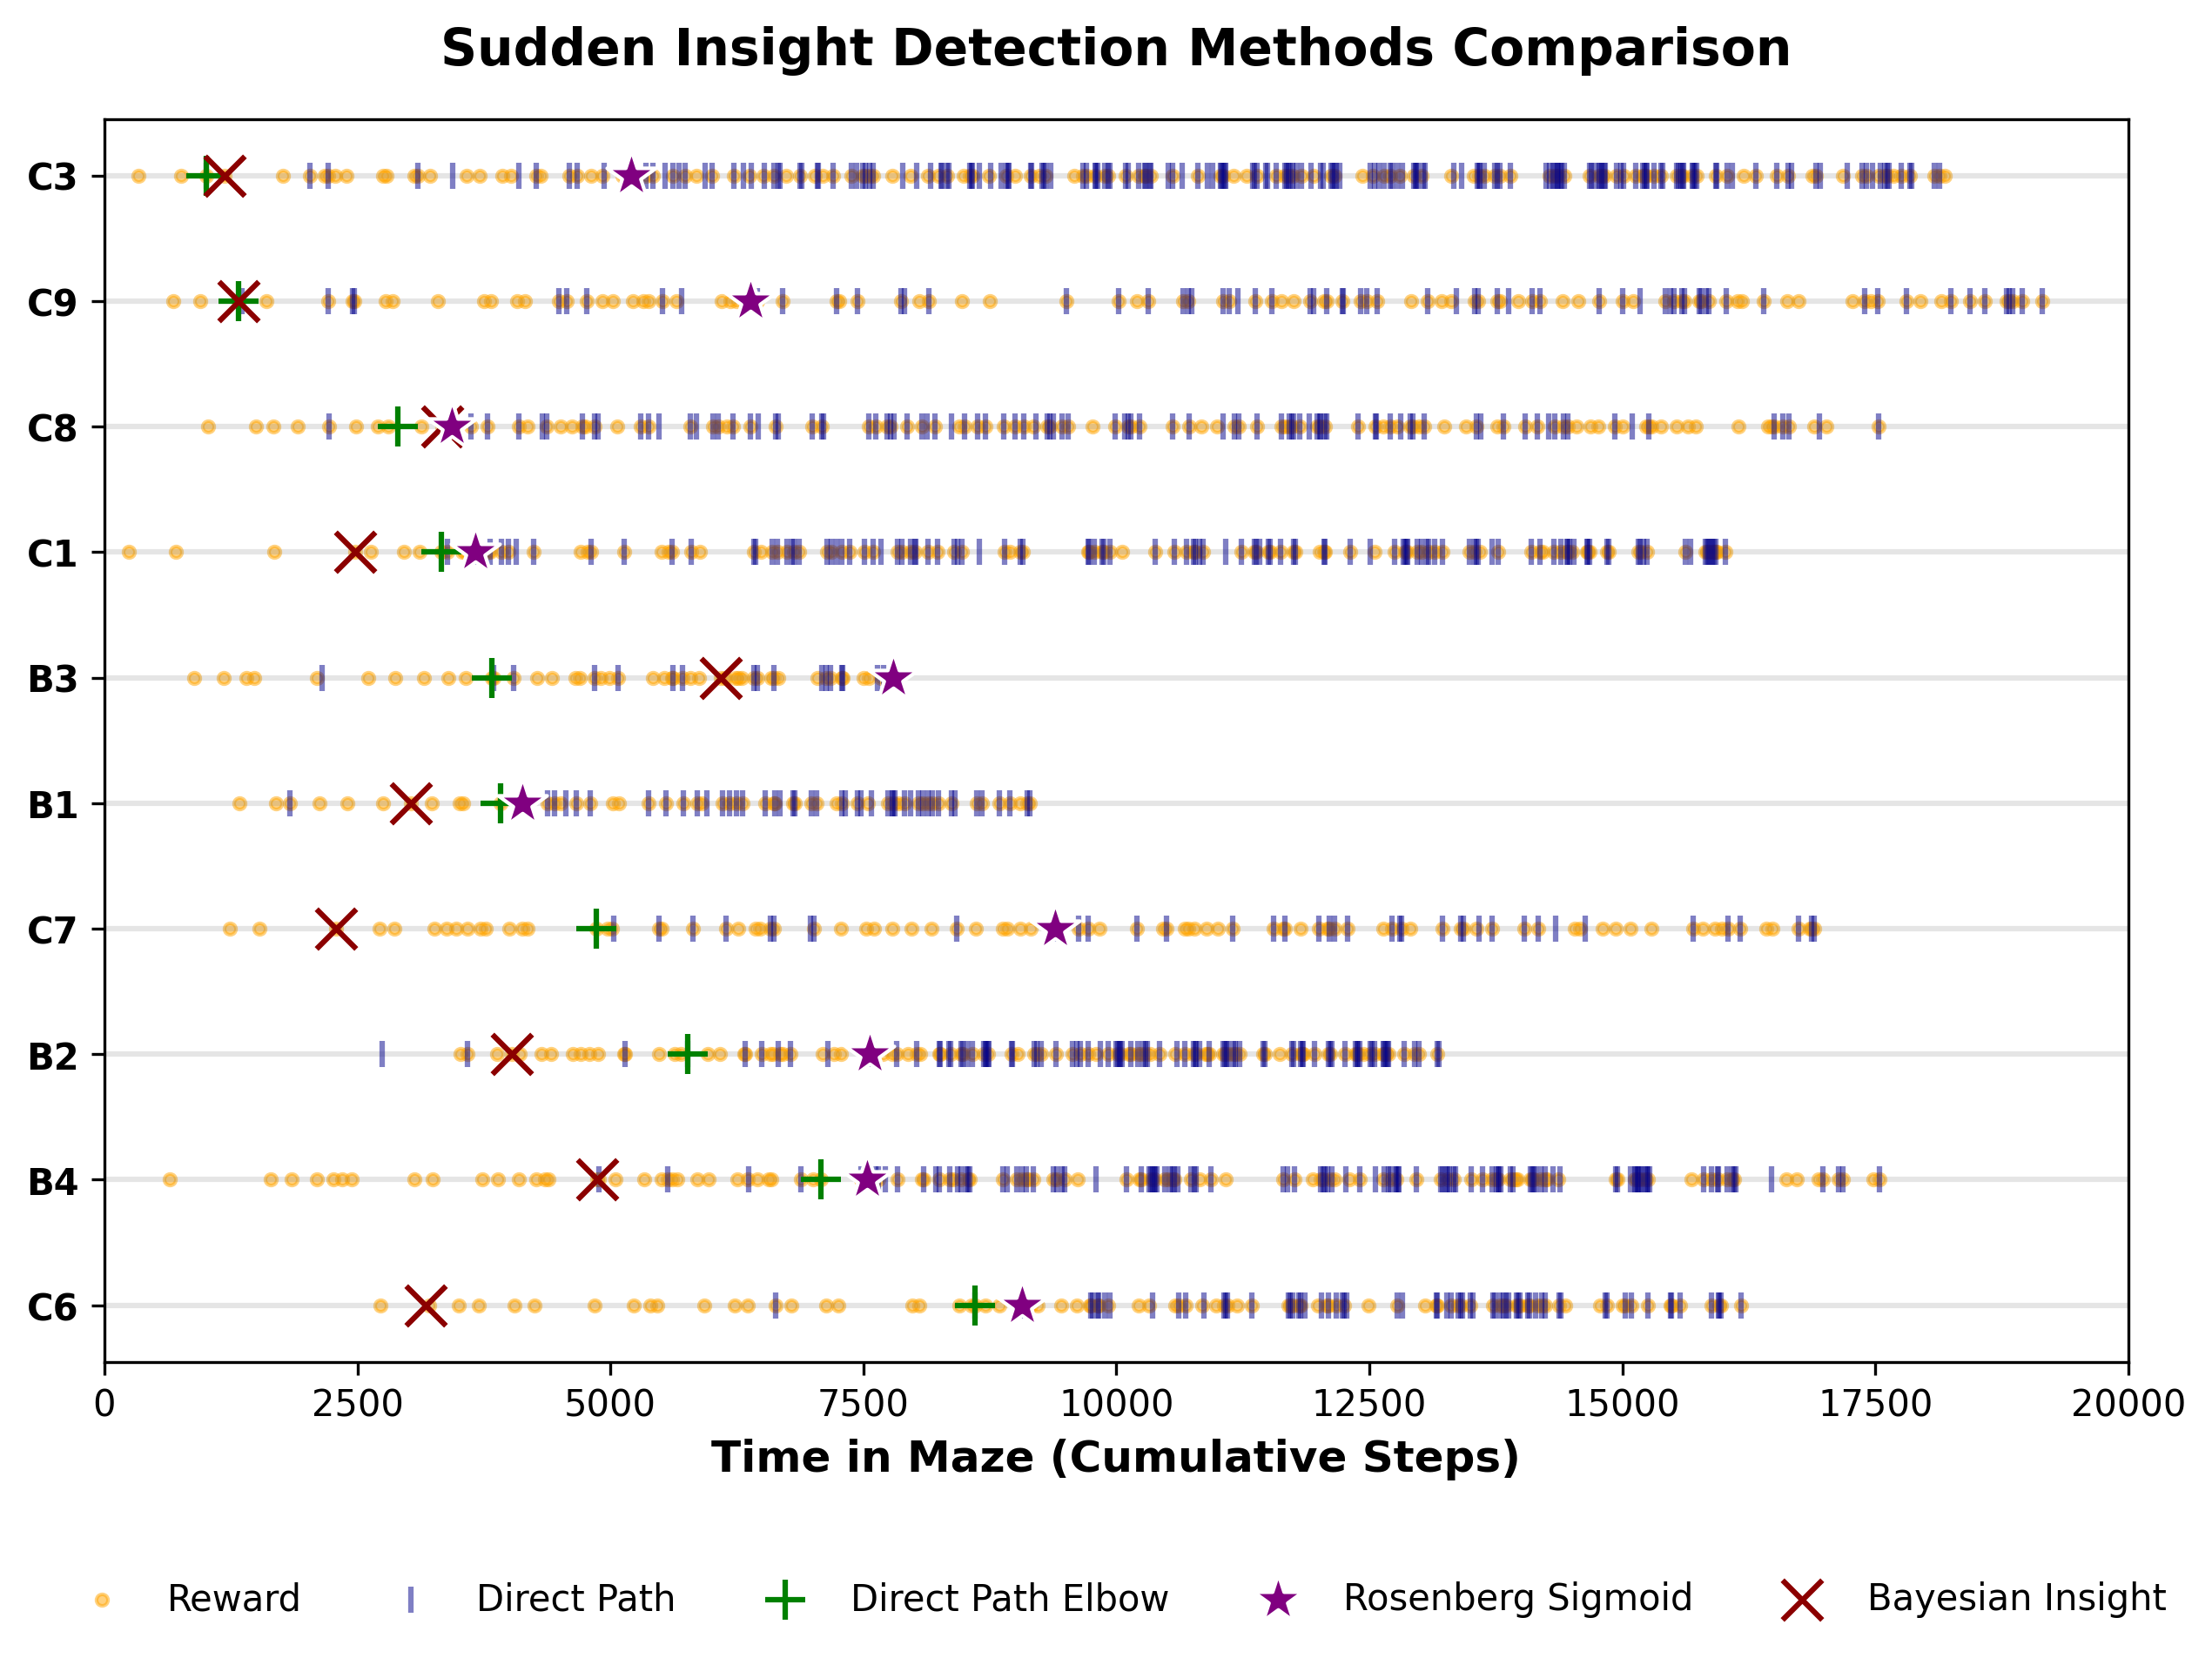
\includegraphics[width=\singlefigure]{figures/sudden_insight_all.png}
    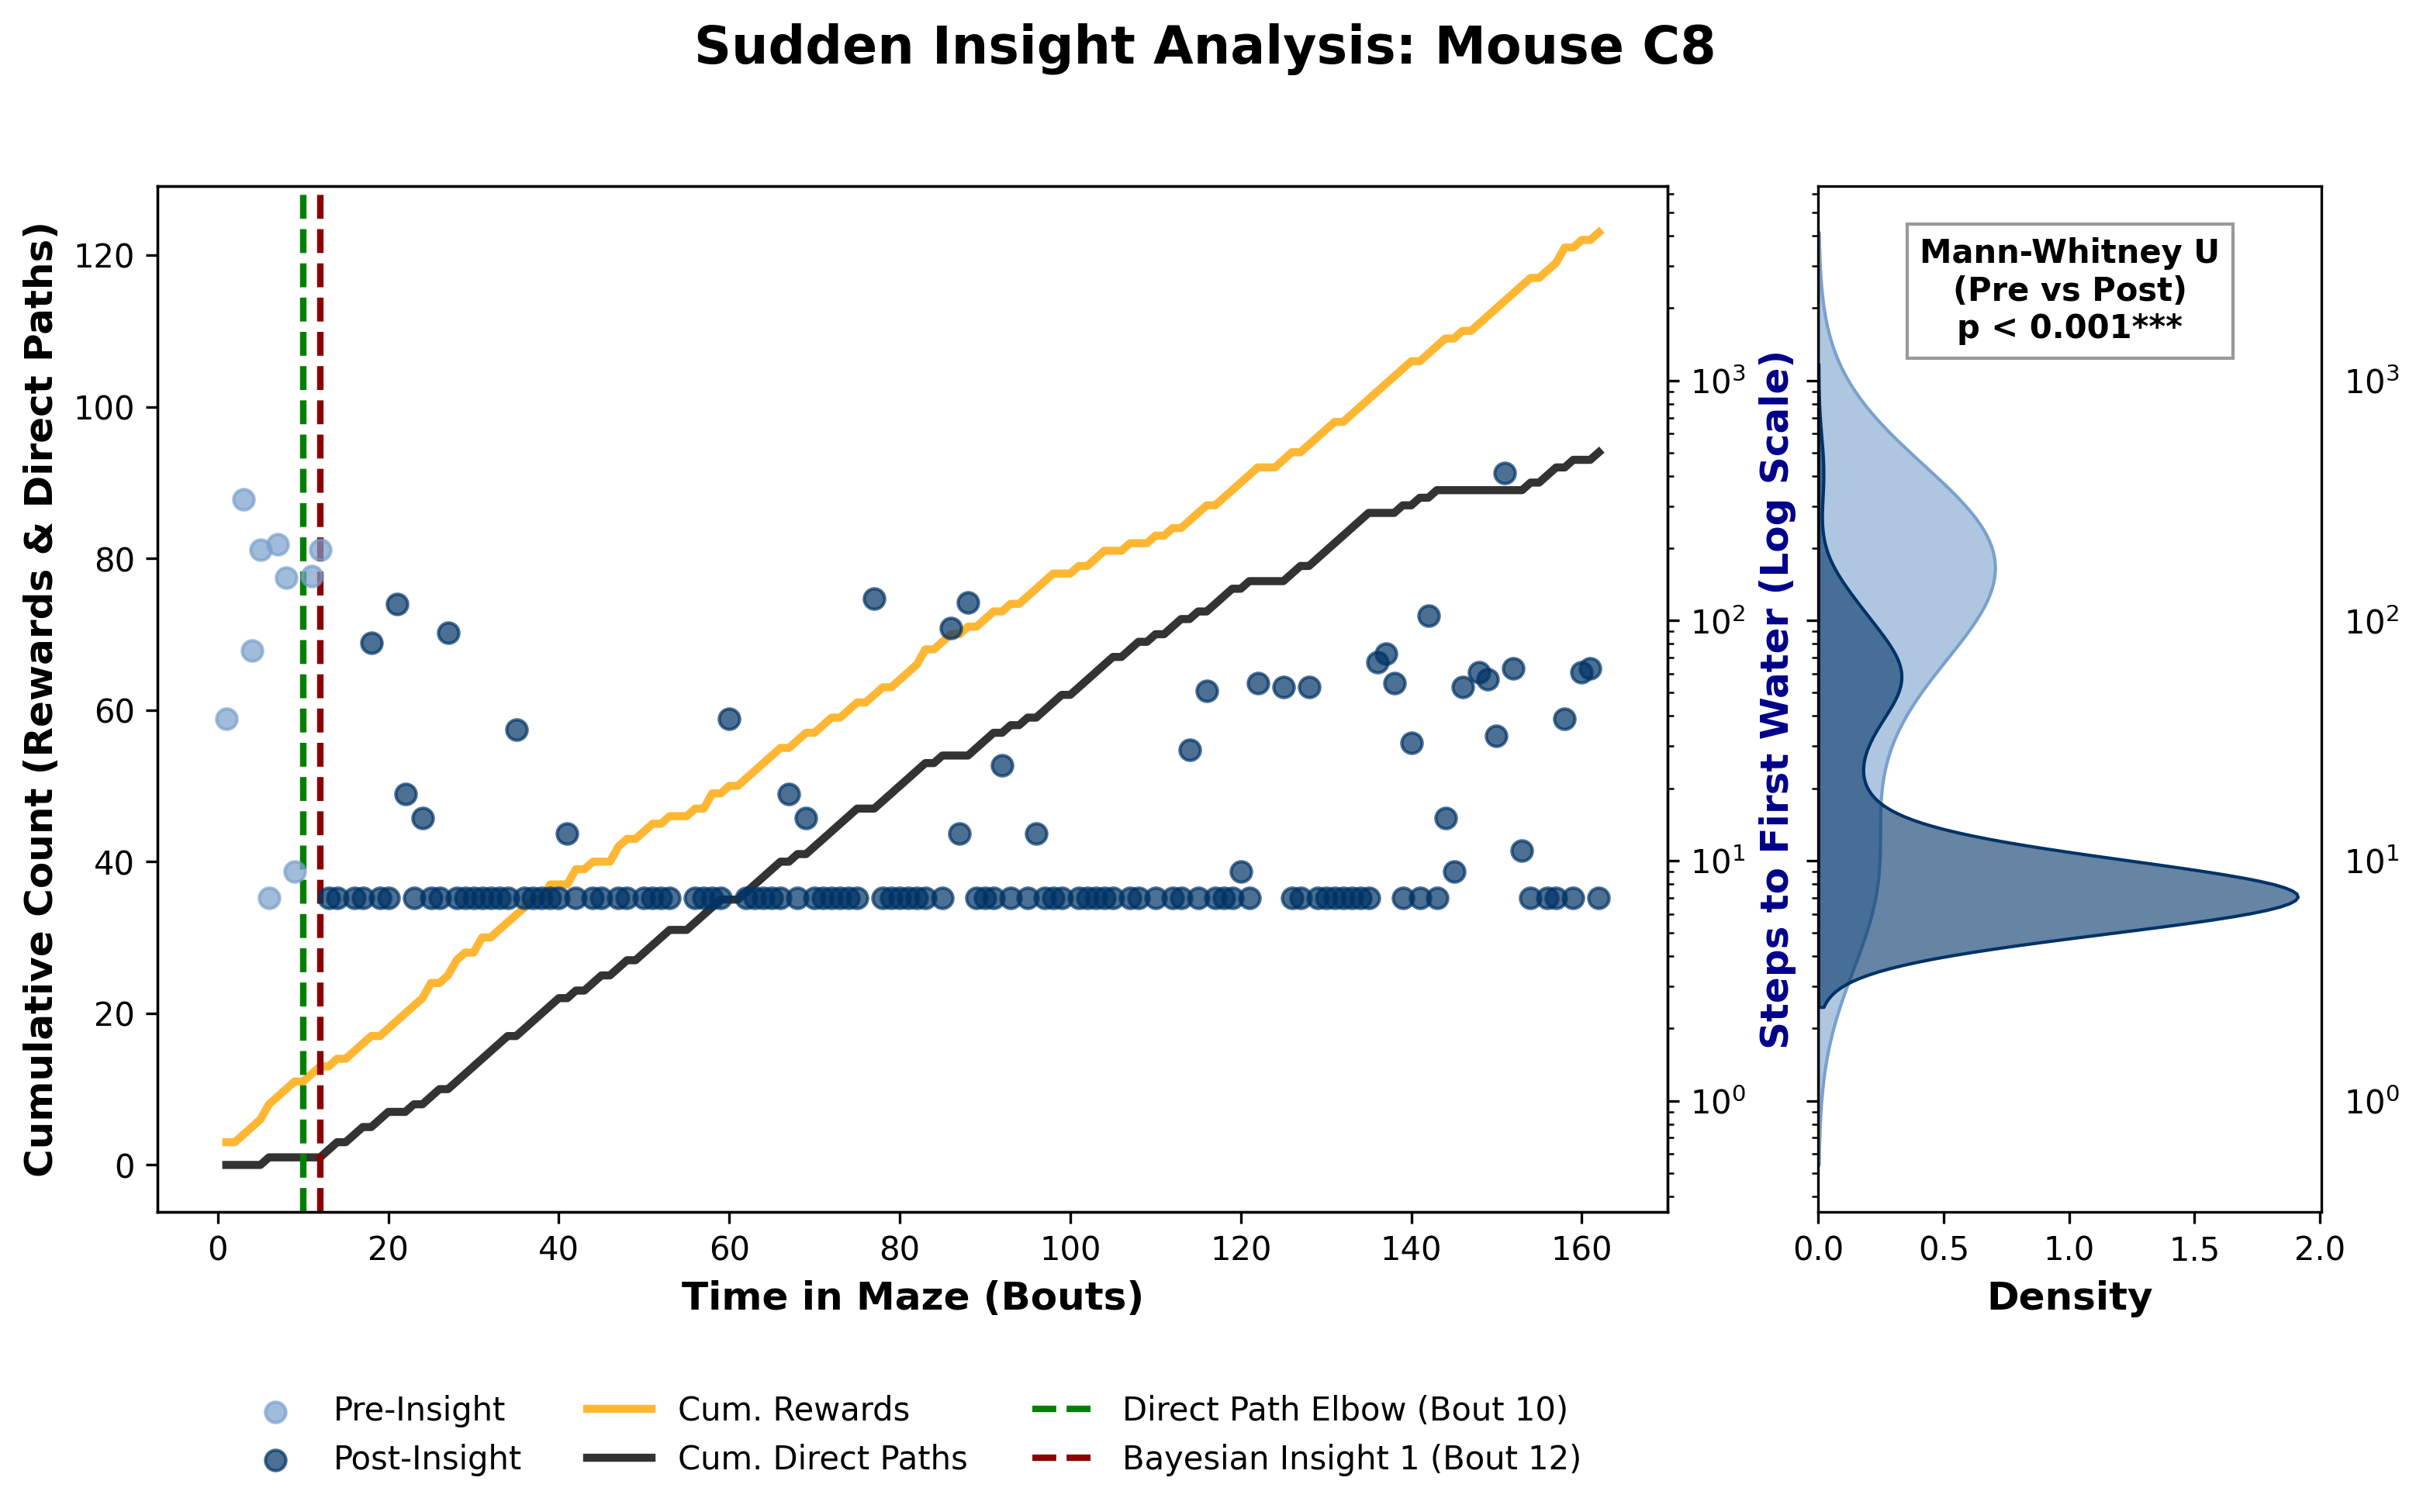
\includegraphics[width=\singlefigure]{figures/sudden_insight_C8.png}
    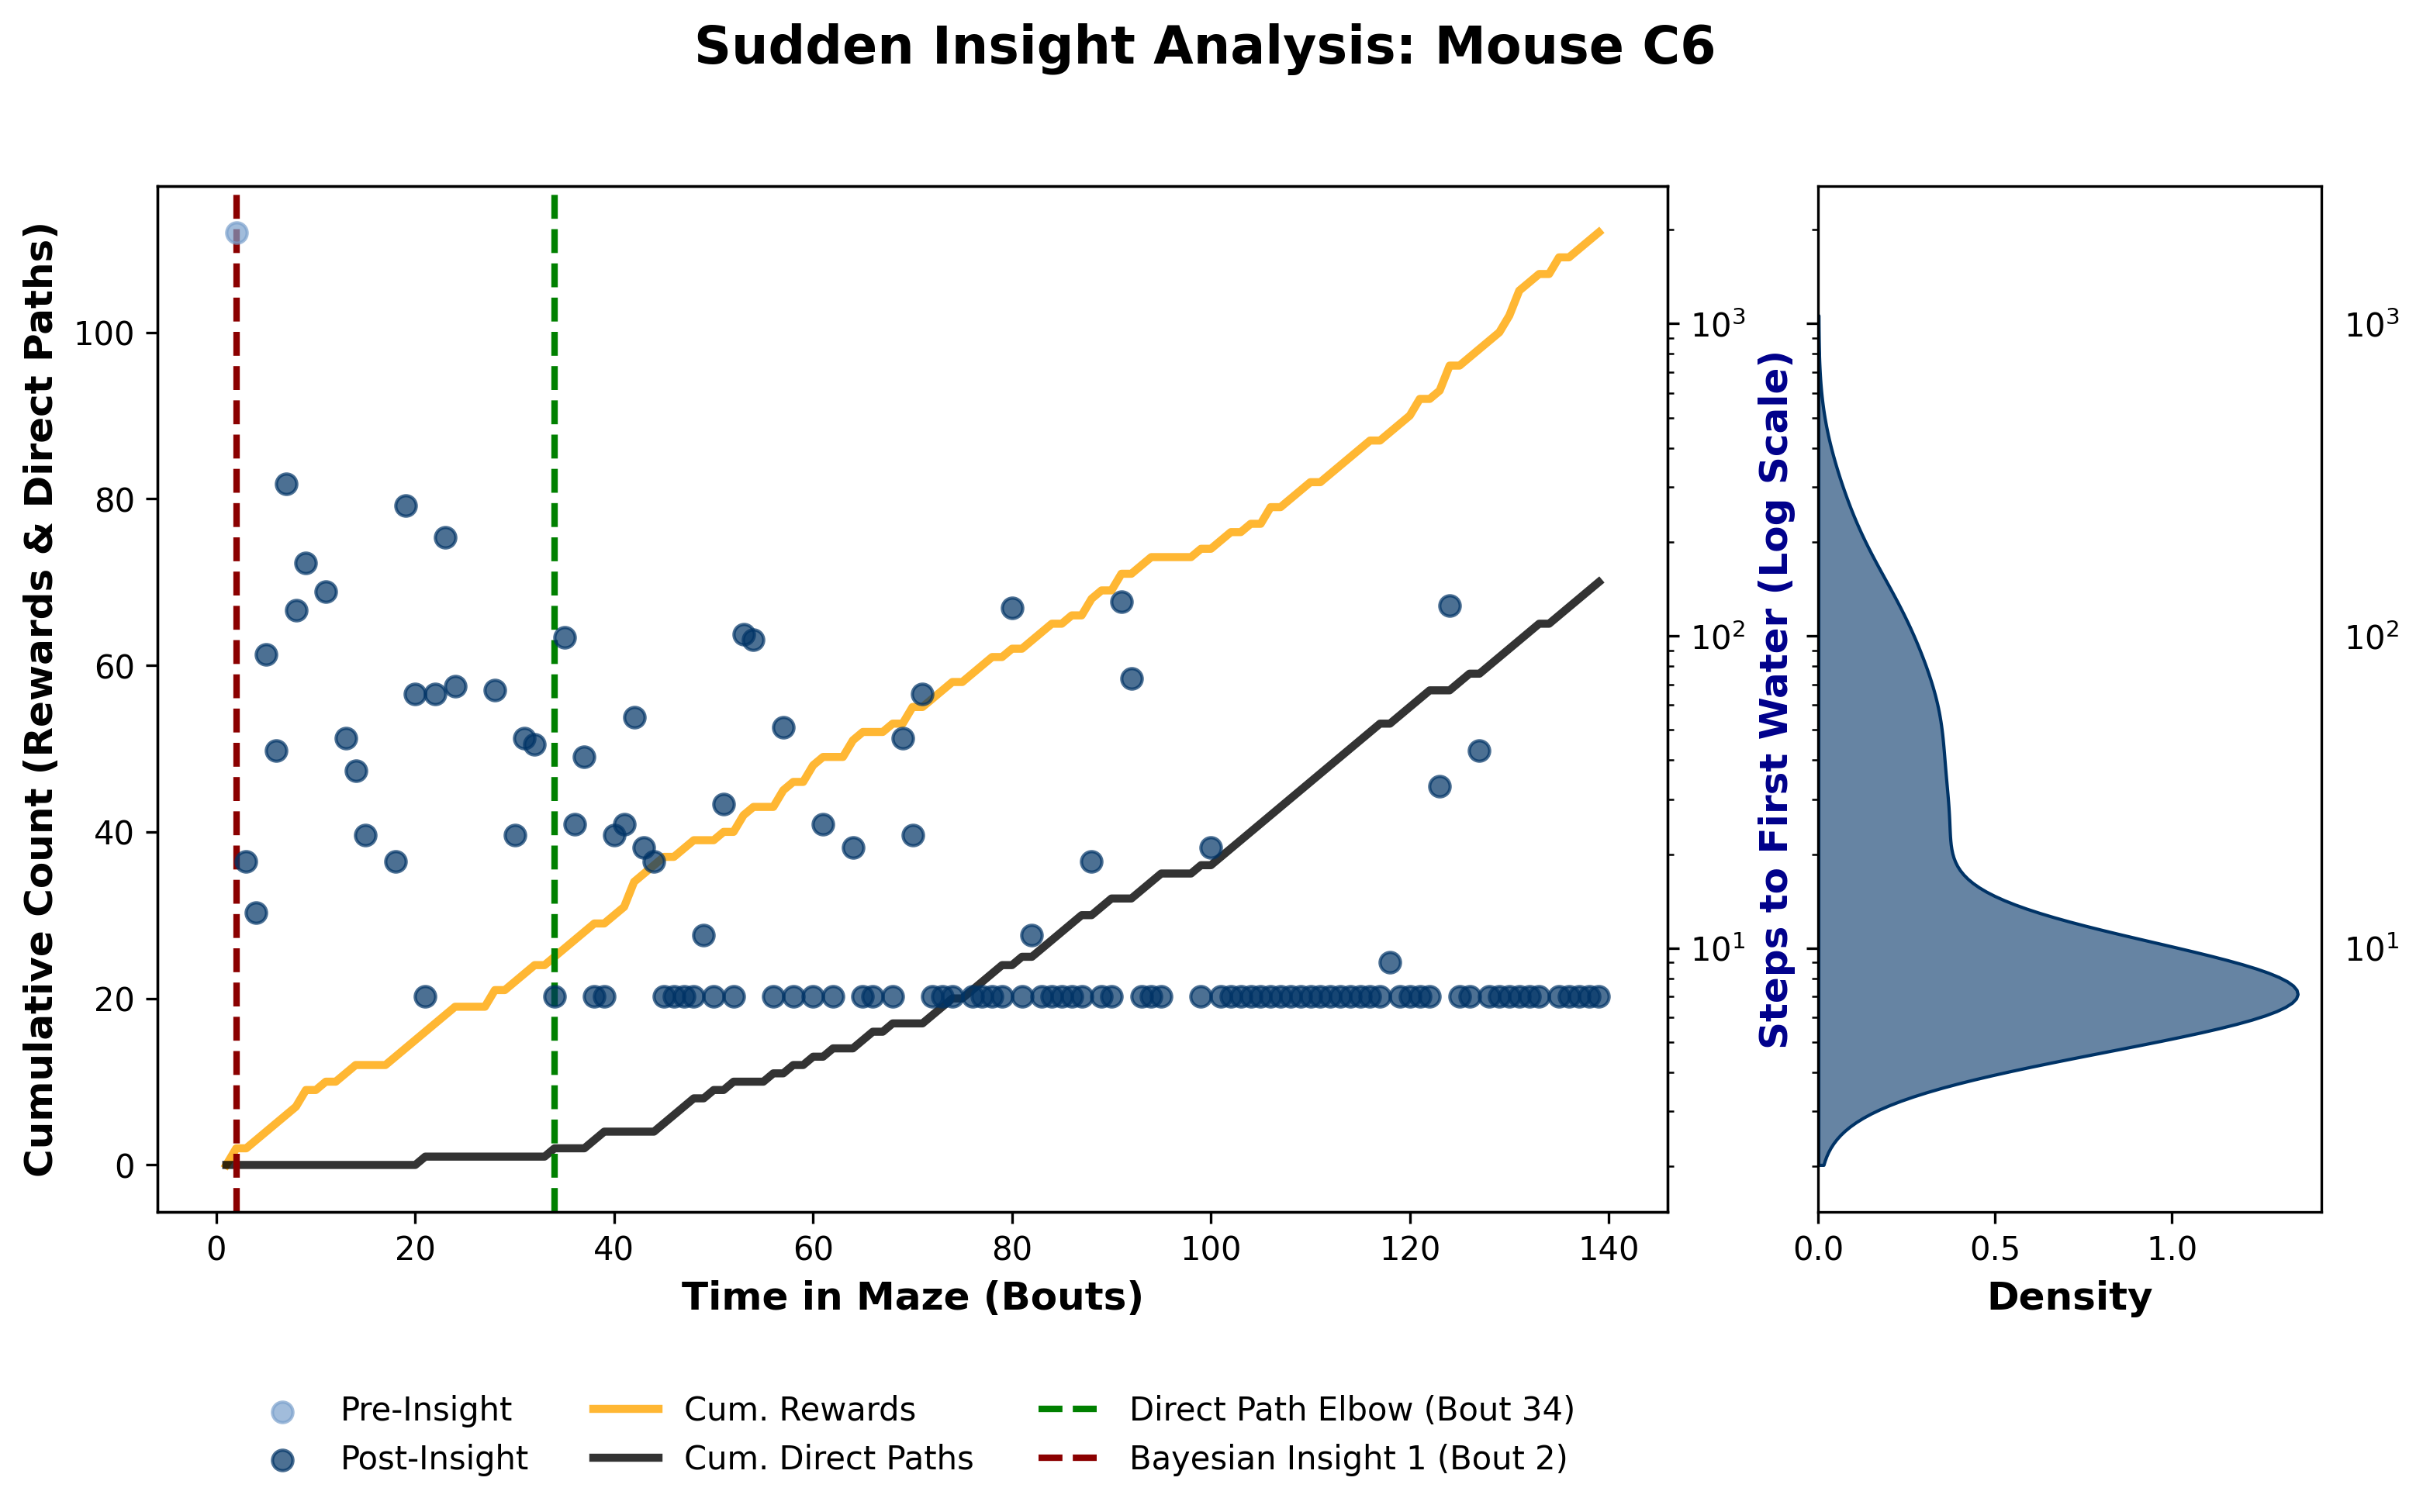
\includegraphics[width=\singlefigure]{figures/sudden_insight_C6.png}
    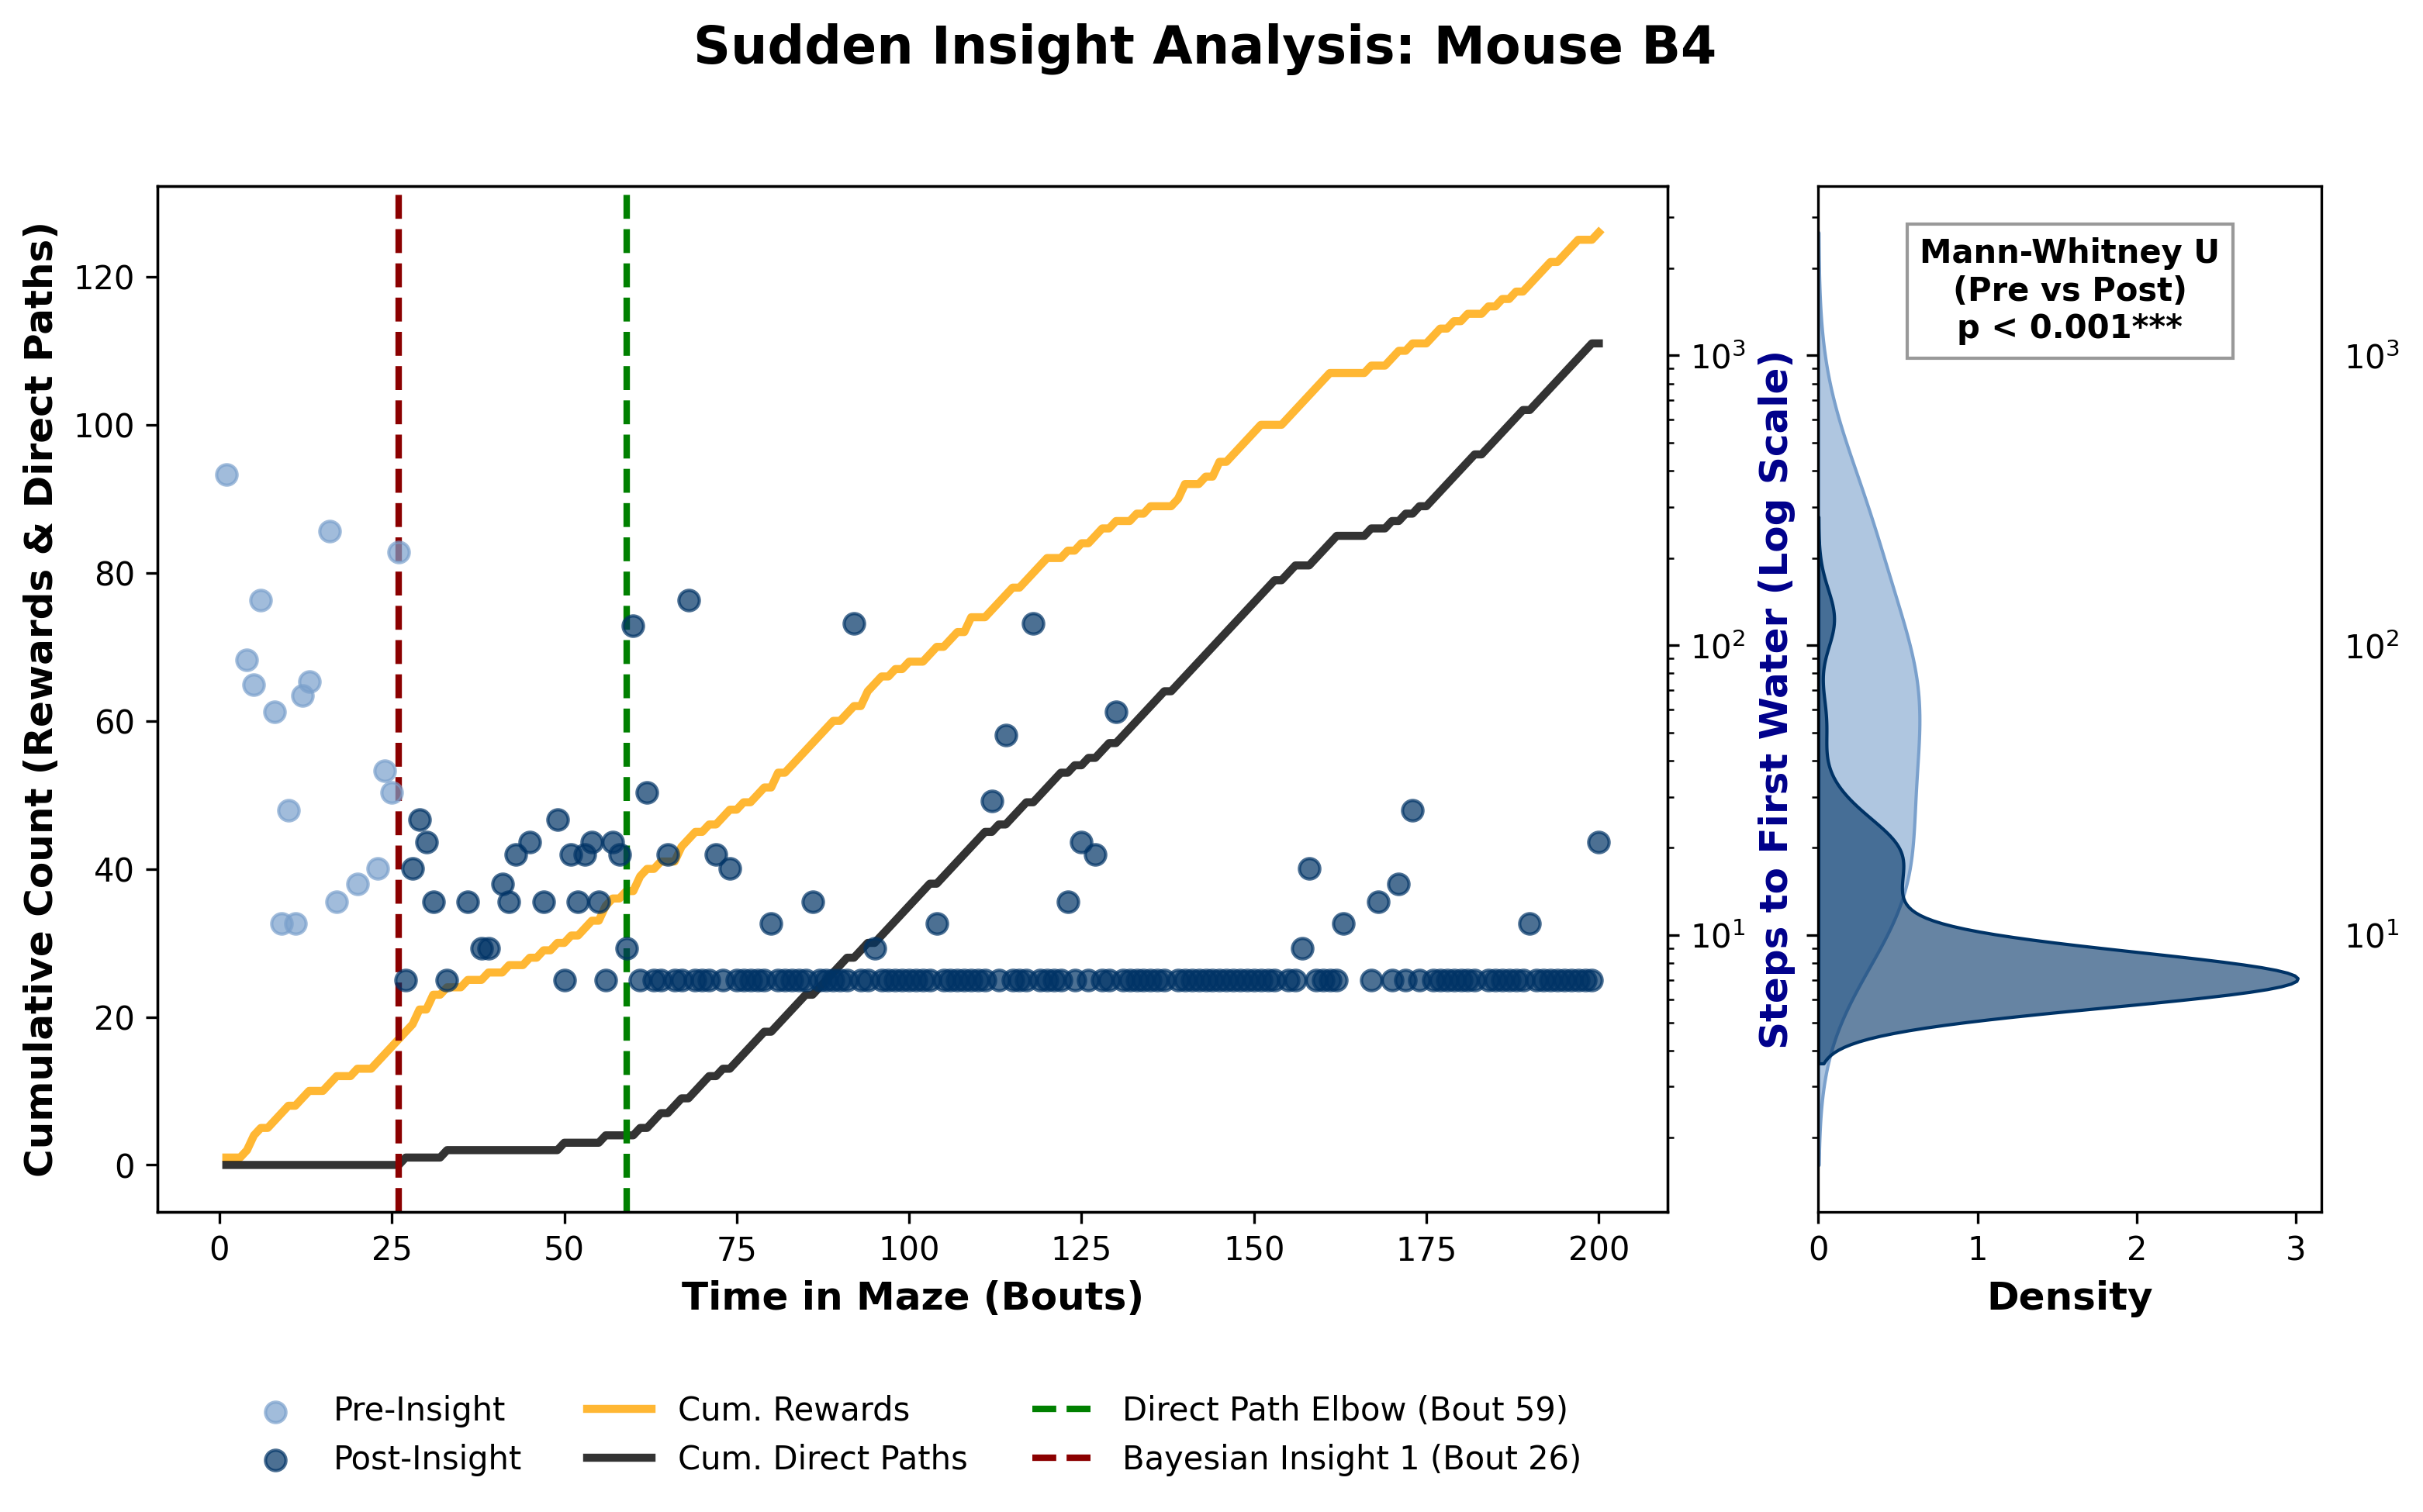
\includegraphics[width=\singlefigure]{figures/sudden_insight_B4.png}
\end{figure}
\section{Behavioural Modes and Latent Target Fixation}
\label{sec:modes_and_fixation}

\subsection{Robustness of Behavioural Modes}
Rosenberg et al. \cite{rosenberg2021mice} proposed that mouse spatial navigation can be partitioned into three distinct behavioural modes: \textit{drink} (direct paths to the water port), \textit{leave} (direct paths to the exit), and \textit{explore} (all other unstructured paths). These modes are assigned deterministically. For example, a trajectory is classified as \textit{leave} if the shortest-path distance to the exit, $d(x_t, E)$, strictly and monotonically decreases with each sequential step $x_t$.

We hypothesised that this strict zero-tolerance rule might be overly sensitive to biological noise, such as brief navigational errors, transient distractions, or minor parsing artifacts in the tracking data. To test the robustness of this classification, we injected a leniency threshold, permitting up to 5 non-monotonic steps before interrupting a \textit{drink} or \textit{leave} sequence. 

Comparing the distribution of behavioural modes over time under both strict and relaxed conditions revealed negligible differences. As shown in Figure \ref{fig:mode_distribution}, the temporal evolution of these modes cleanly reproduces the findings of Rosenberg et al. \cite{rosenberg2021mice}, transitioning from purely exploratory behaviour to a stable exploitation-driven regimen. We therefore conclude that the deterministic routine is highly robust to transient navigational noise.

\begin{figure}[htbp]
    \centering
    % Replace with your actual filename for the modes over time plot
    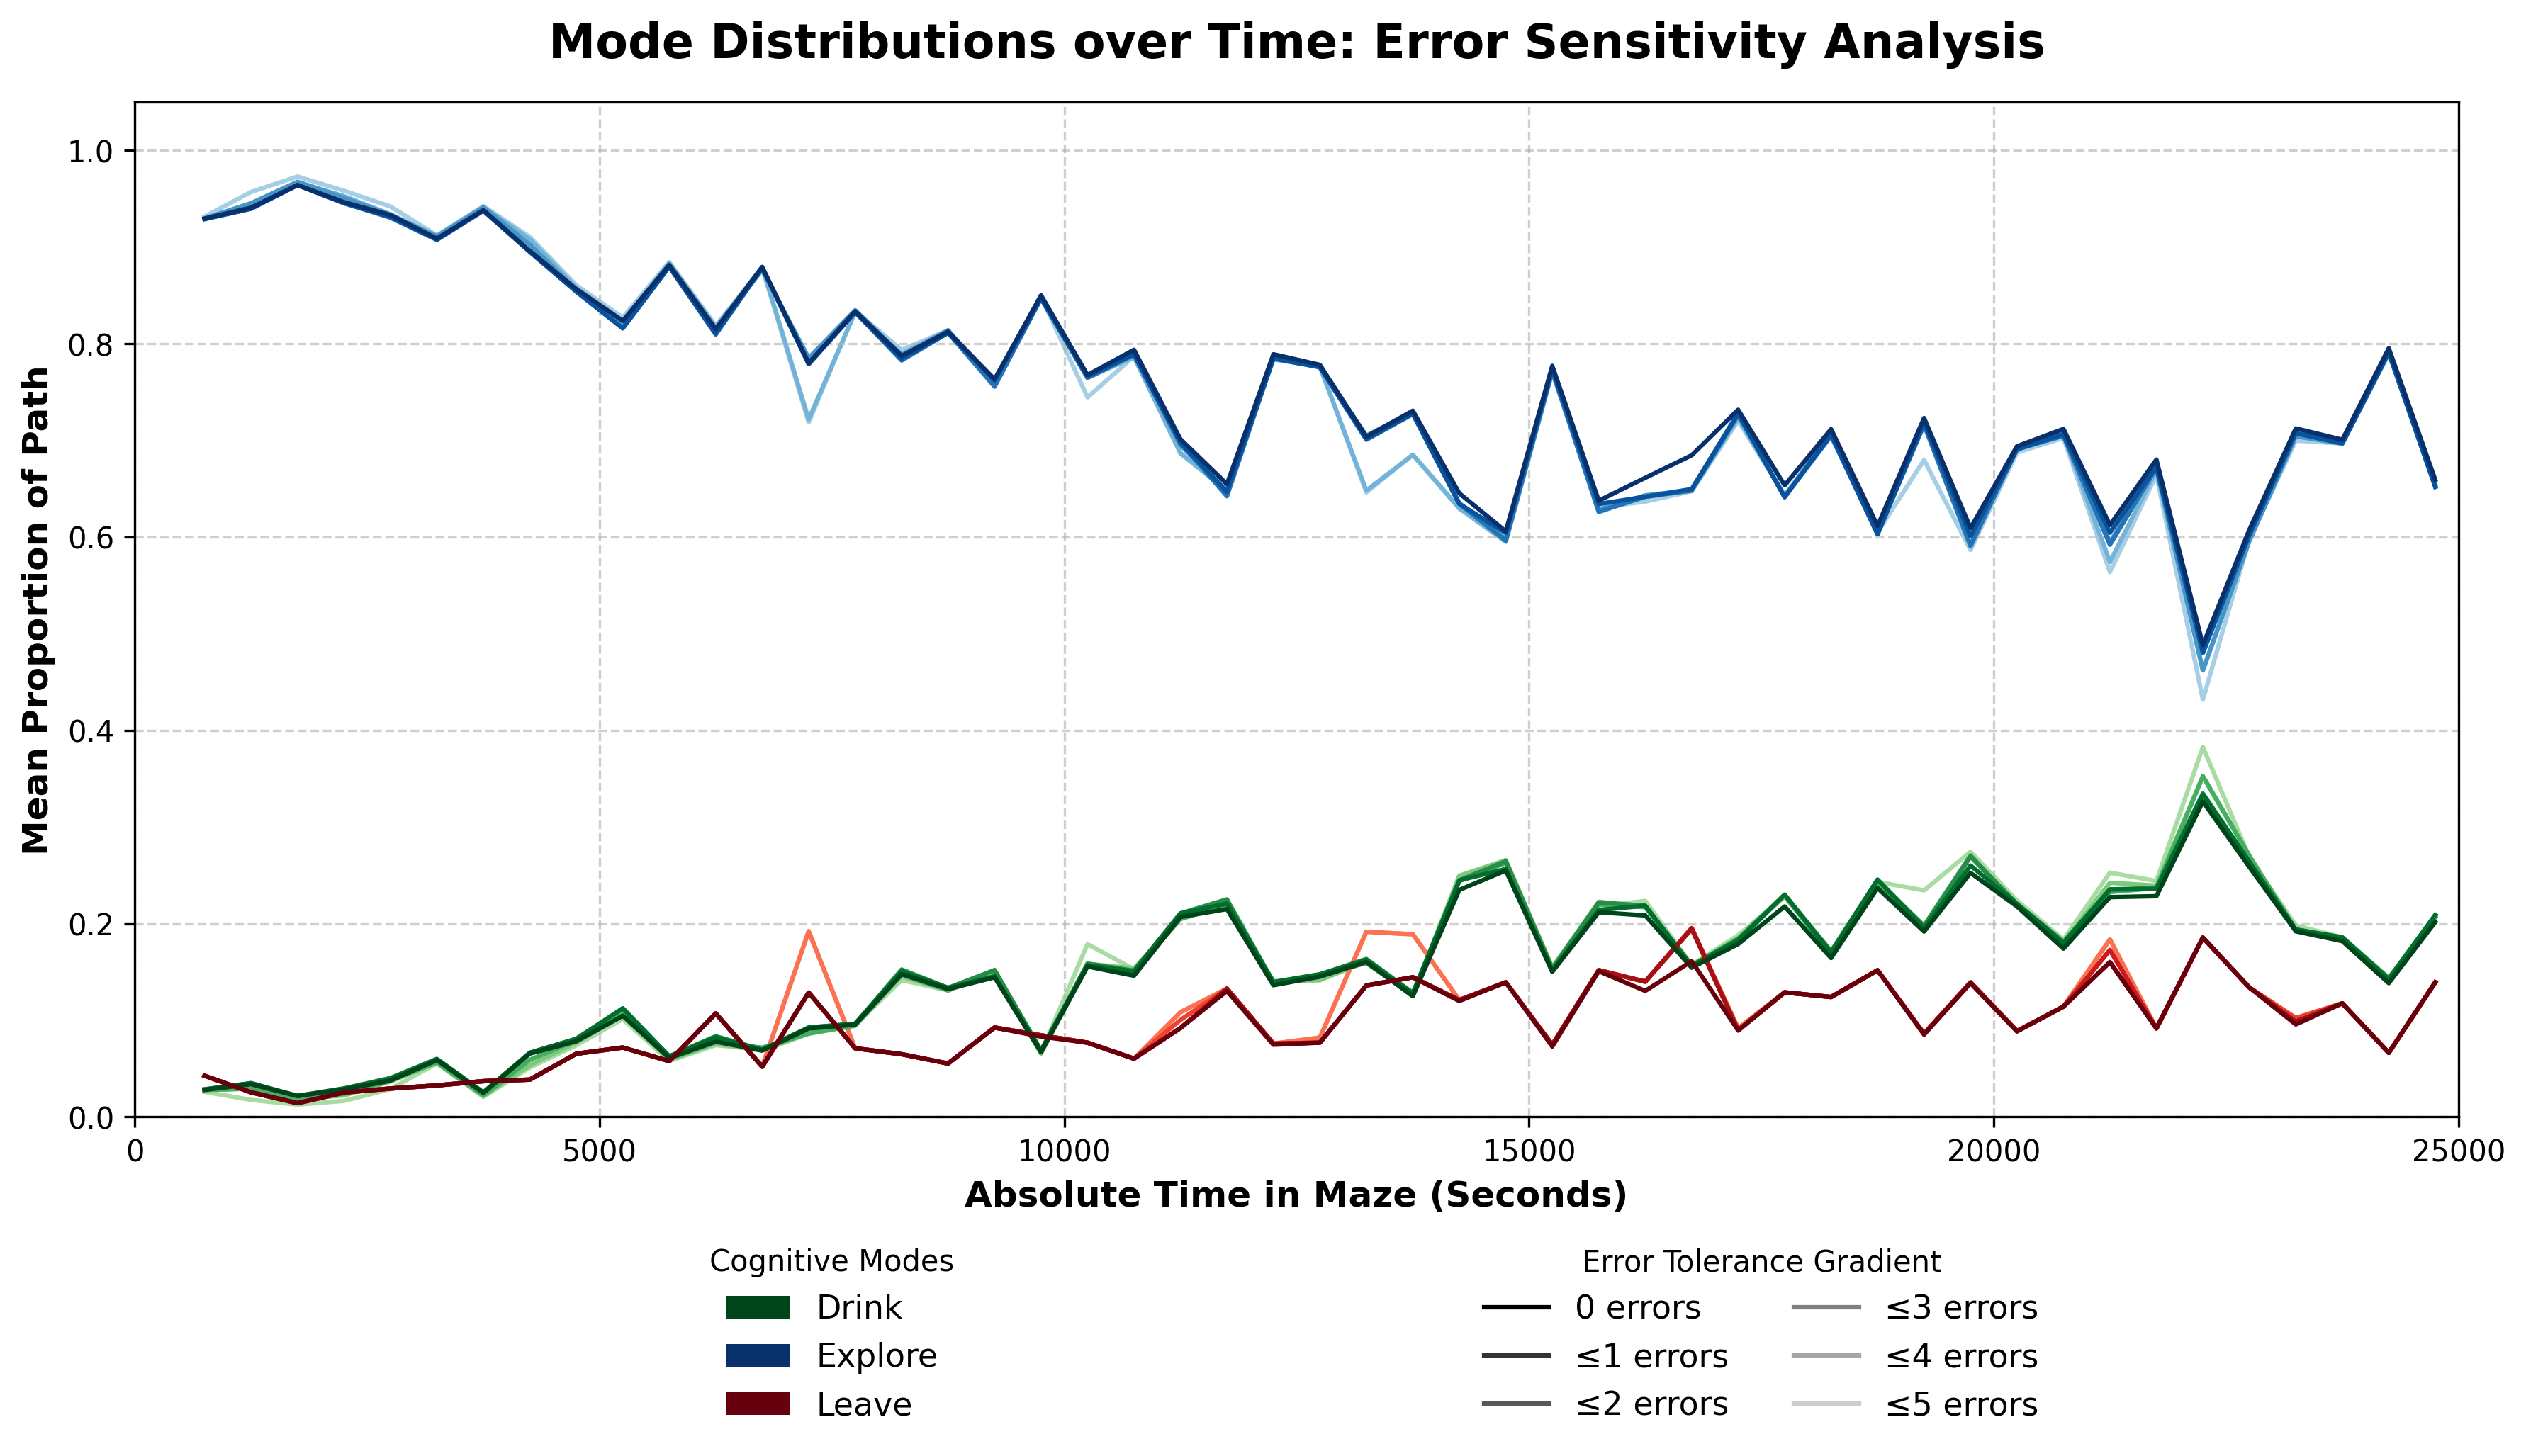
\includegraphics[width=0.48\textwidth]{figures/mode_sensitivity.png}
    \caption{\textbf{Distribution of Behavioural Modes Over Time.} Mean Behavioural mode proportion across mice, plotted over time. Tolerances shown by decreasing shade of respective mode colours for explore (blue), drink (green), leave (red)}
    \label{fig:mode_distribution}
\end{figure}

\subsection{Unrewarded Target Fixation and Short Paths}
While the three generic modes capture broad behavioural states, analysing the specific spatial distribution of unstructured \textit{explore} bouts reveals highly non-uniform tendencies. As shown in Figure \ref{fig:leaf_visits}, both the rewarded and unrewarded groups exhibit a strong baseline preference for exploring the extreme corners of the maze, followed by the outer edges, with internal nodes receiving the least attention.

However, Nodes 115 and 116 represent significant outliers to this spatial gradient. Node 116 houses the water port apparatus. Crucially, the unrewarded group exhibits a pronounced preference for investigating this specific node, despite never receiving a water reward. We propose two hypotheses for this latent target fixation: (1) residual olfactory markers left by the rewarded group despite cleaning protocols, or (2) the physical irregularity of the dry water spout acting as an inherent point of investigatory interest within an otherwise uniform maze.

\begin{figure}[htbp]
    \centering
    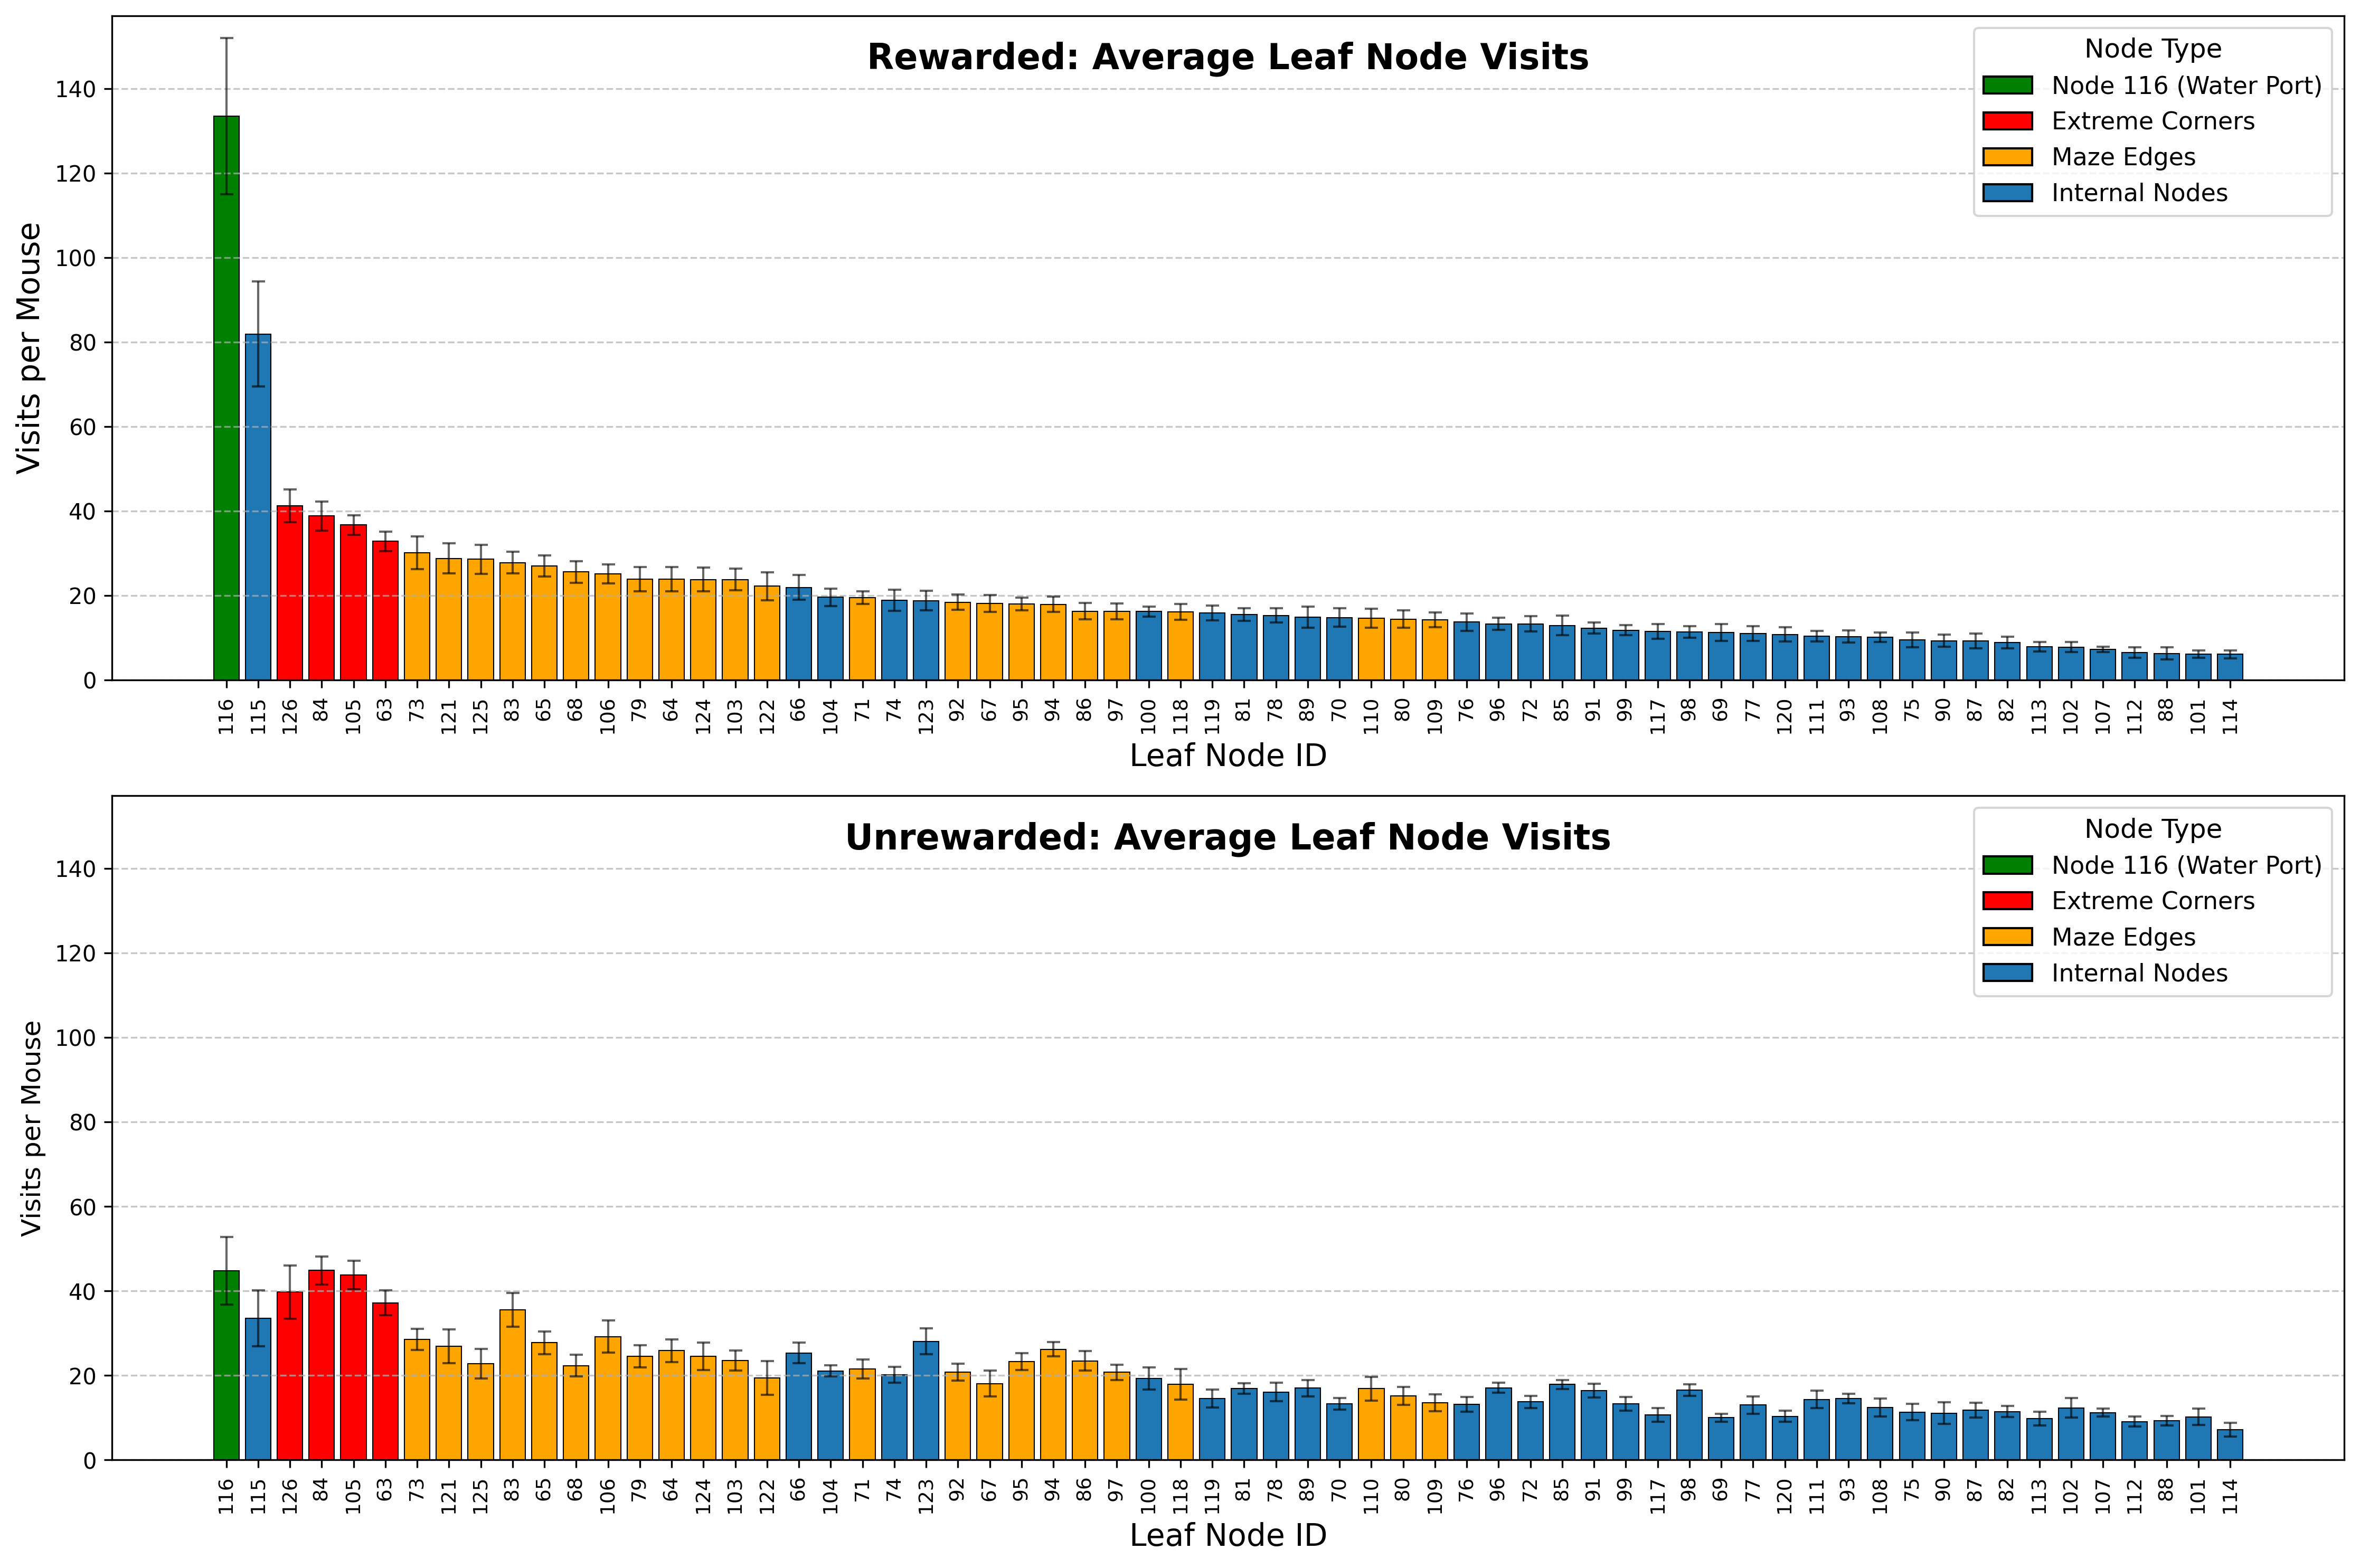
\includegraphics[width=0.5\textwidth]{figures/leaf_node_visits.png}
    \caption{\textbf{Average Leaf Node Visits.} Frequency of visits to maze leaf nodes. Both groups display a geometric preference for extreme corners (red) and edges (orange) and the water port (Node 116, green).}
    \label{fig:leaf_visits}
\end{figure}

To determine whether these visits to Node 116 were random anomalies or structured behaviour, we conducted a spatial and kinematic analysis of recurring ``short paths'', sequences of steps that mice repeat taking direct paths from home to an apex node, before returning home. Though there is no obvious pattern to these short bouts, they reveal behaviours distinct from the three modes defined. 

Our analysis of the dwell times (node duration) during these specific paths reveals a distinct kinematic signature. We partitioned these trajectories into three phases: the \textit{outbound} journey, the \textit{apex} (the deepest point of the path), and the \textit{inbound} return. As demonstrated in Figure \ref{fig:short_paths}, the mean dwell time is larger at the apex of these short paths across both groups, though still far lower than for visits to the water port.

This kinematic pausing strongly supports the hypothesis that these are not artifacts of random wandering, but rather directed investigatory ``short bouts'' or patrolling behaviours. The presence of this highly structured, goal-oriented movement within the theoretically unstructured \textit{explore} dataset suggests that future work may need to classify a fourth behavioural mode to accurately partition directed investigation from pure random exploration.

\begin{figure}[htbp]
    \centering
    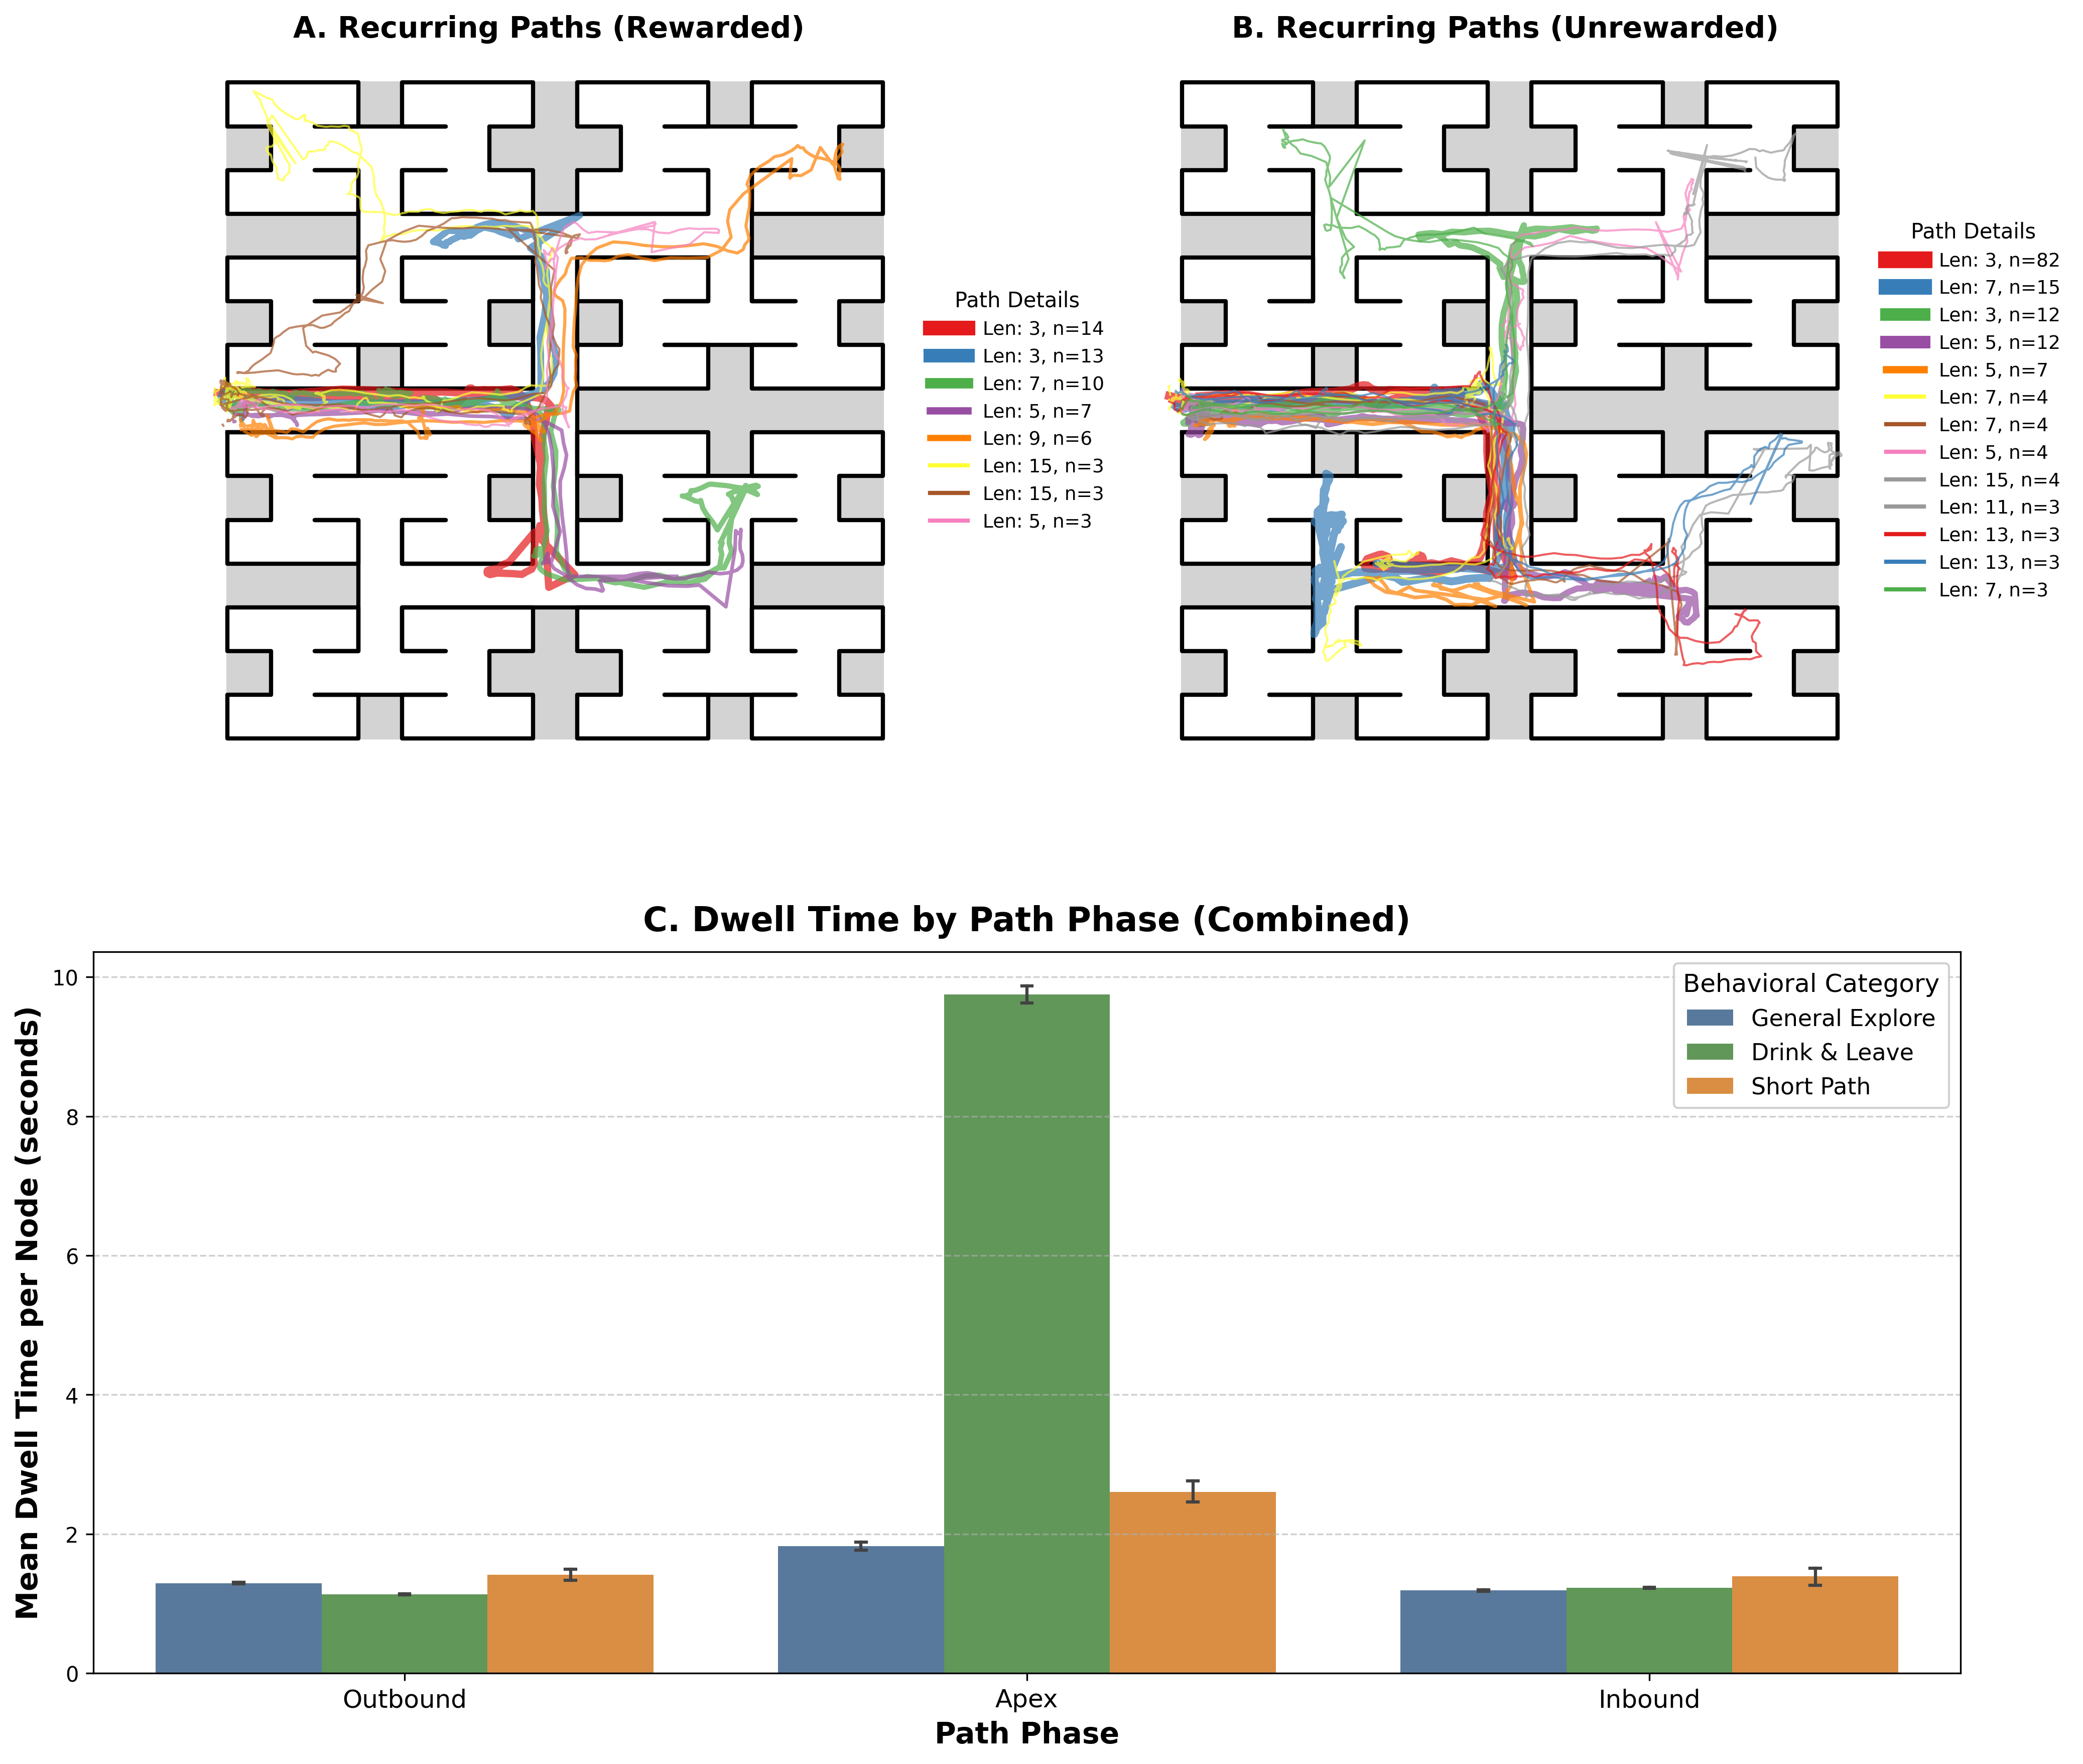
\includegraphics[width=0.5\textwidth]{figures/short_paths.png}
    \caption{\textbf{Spatial and Kinematic Profile of Recurring Short Paths.} (A, B) Analysis of node dwell times across modes and path phases. Three phases are defined: outbound, apex, and inbound. Trajectories categorised as exploration (blue), drink (green) and investigative short paths (orange).}
    \label{fig:short_paths}
\end{figure}
\section{Do Rewards Bias Exploration?}

\subsection{Modelling Exploration}
\begin{itemize}
    \item Rosenberg impements a markov chain model to for exploration behaviour. This model effectively memorizes turning statistics. 
    \item Across mice they observe four biases in node action decisions as follows:
    \item <insert description of biases>
    \item They implement a simplified 4-bias markov model and train these on each mouse to determine a weighting for each bias which reflects the mouses tendencies during exploration.
    \item We explore these models with respect to both
    \item a) the influence of maze and reward structure on exploratory behaviour,
    \item b) the generality of the different models
    \item The 4 biases are given as follows:
    \item 2 biases covering movement deeper into the maze: $P_{SF}$ is the probability that the mouse will move forward. $P_{SA}$ that it will alternate left and right actions at a T junction. 
    \item 2 biases covering movement out of the maze: $P_{BF}$ is the probability that the mouse will move forward through the junction. $P_{BS}$ that it will turn rather than go straight.
    \item The direct path from home to water port is achieved by the following sequence of actions: RLLRLR, where R is right and L is left
    \item While the direct path from water port to home is given by the sequence: STTTTTT, where S is straight, and T is turn
    \item We see that for the direct path to water, $P_{SF} = 1$ and $P_{SA} = 0.8$. Identically for the direct path home, $P_{BF} = 1$ and $P_{BS} = 0.8$.
    \item Thus drink and leave modes should have high values for these biases, and we observe this in <insert figure >
\end{itemize}

\begin{figure}
    \centering
    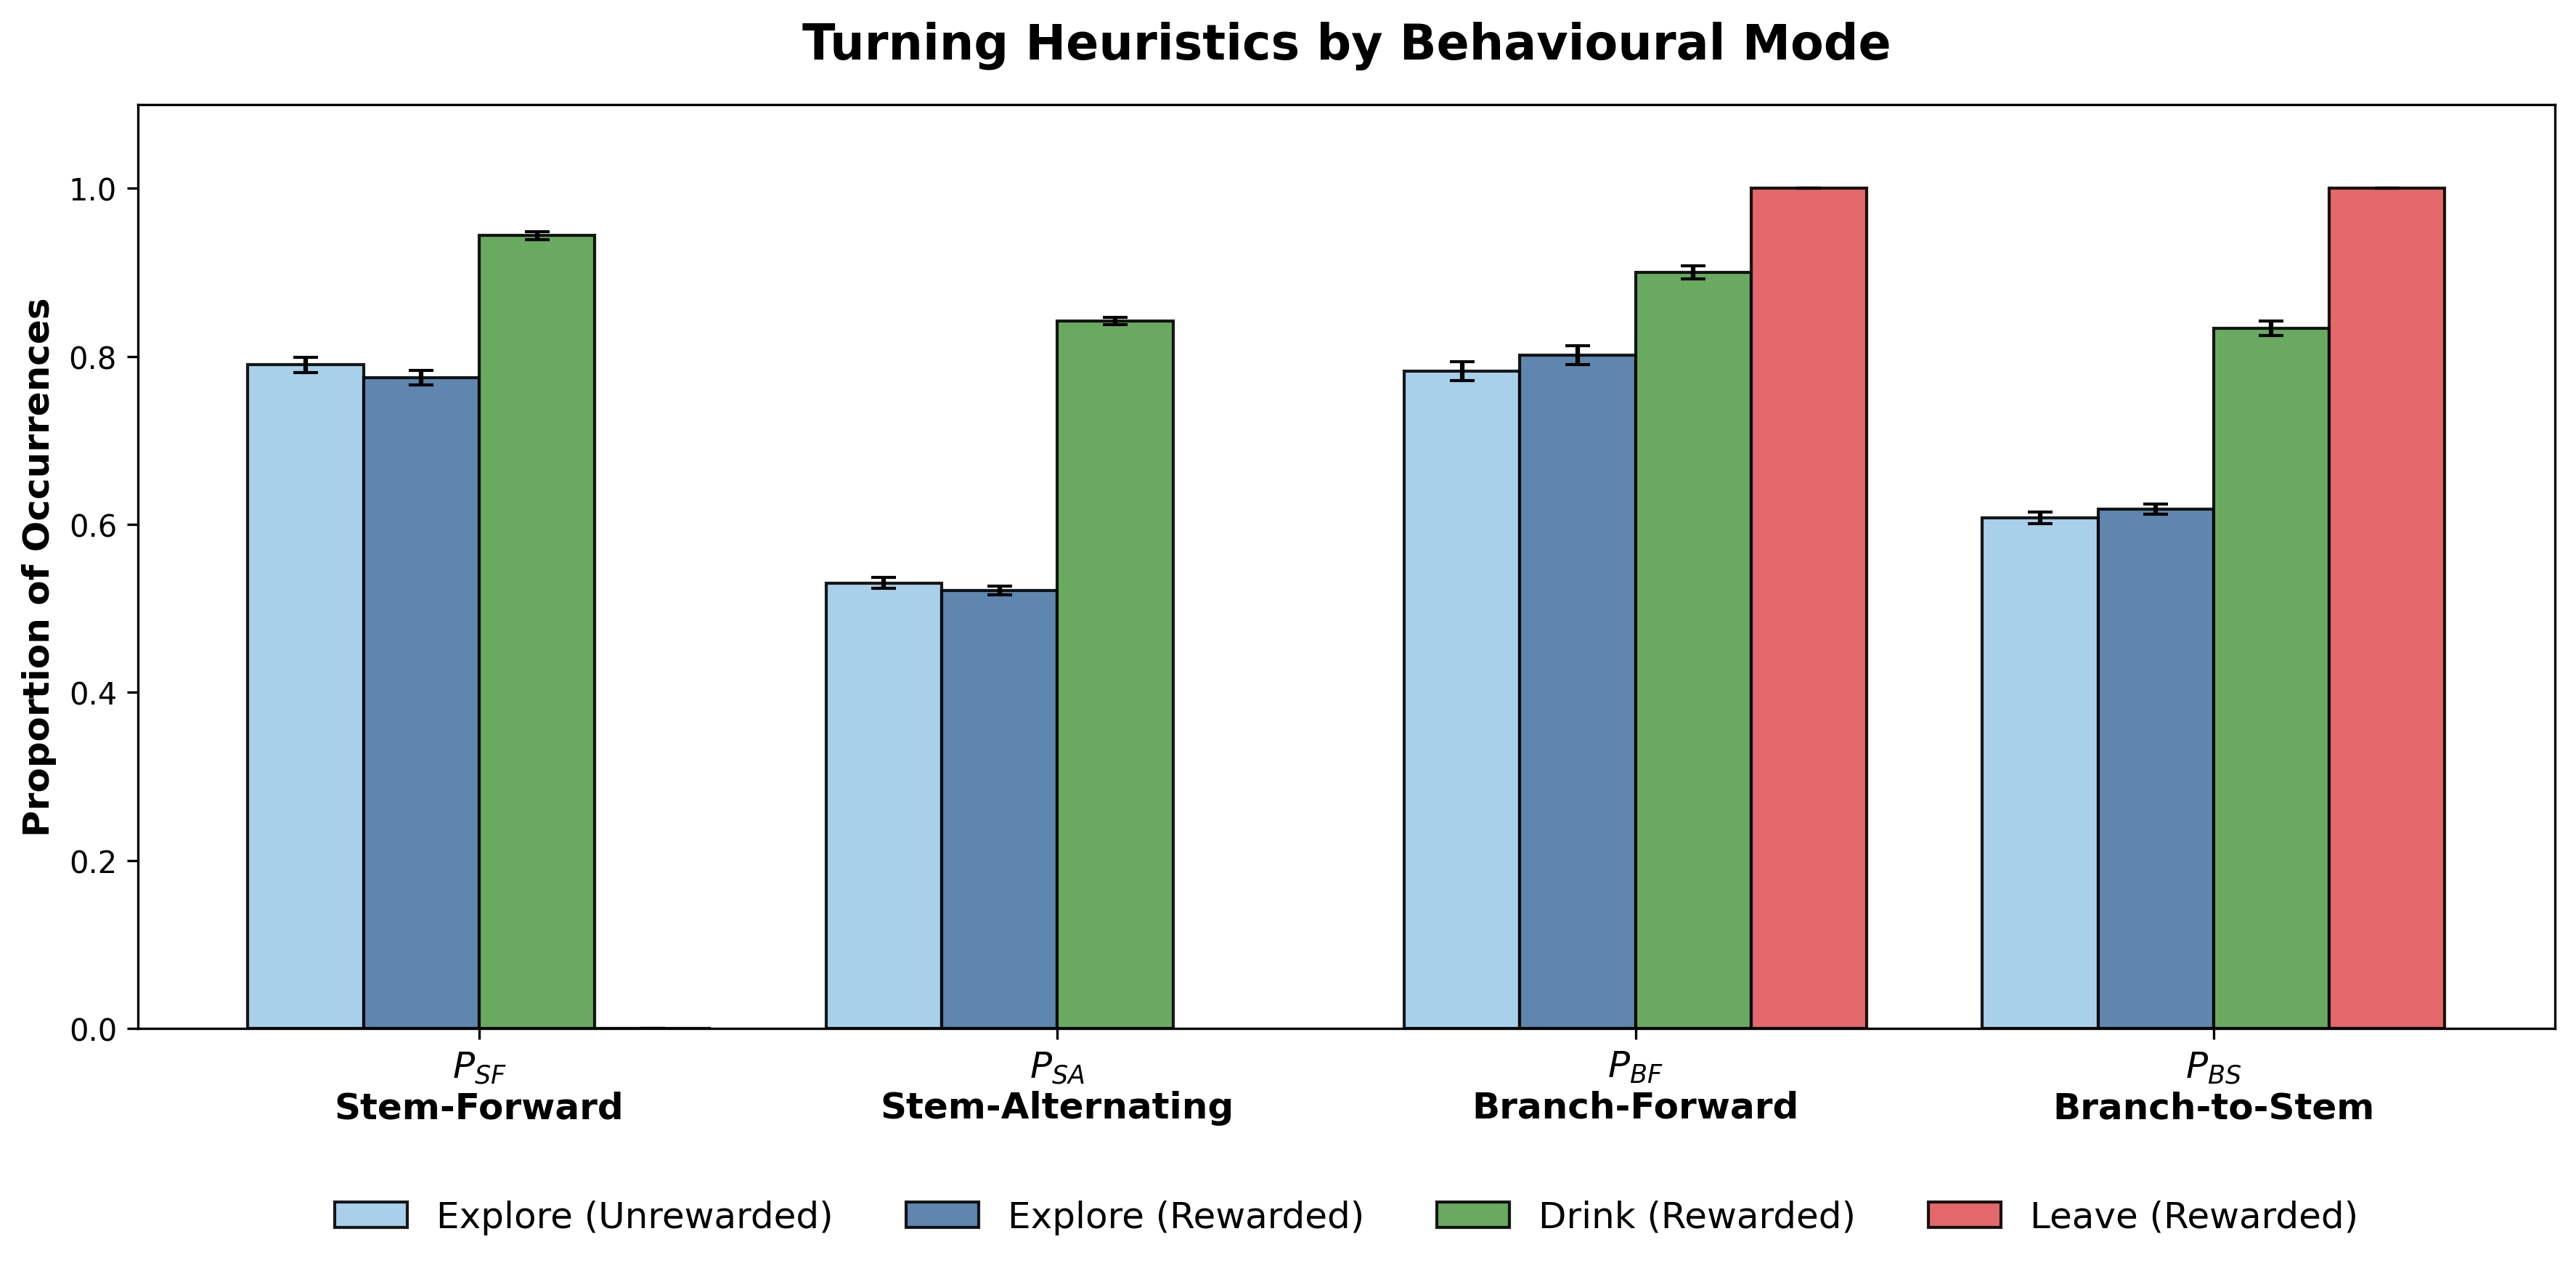
\includegraphics[width=\singlefigure]{figures/heuristics_by_behavioural_mode.png}
\end{figure}

\subsection{Do Models Generalise?}

\begin{itemize}
    \item We test the generalisaibility of the 4-bias models. We train one model per mouse on explore mode data for both rewarded and unrewarded groups. 
    \item We train them using a 5-fold cross validation, and test each model on each mouse by calculating the cross-entropy of model predictions against the 20\% test data and use a box plot to analyse the results.
    \item We make a number of observations. 
    \item For both groups, the cross-entropy has a range of 0.1, suggesting that there is a range of structured behaviour in exploration.
    \item The unrewarded mice tend to have a higher cross-entropy, suggesting that their exploration is more random.
    \item We also observe that models trained on the unrewarded mice generally perform better on the rewarded mice than on the target of training, again suggesting more randomness in exploration for unrewarded mice.
    \item Variance in cross-entropy of models trained on differnet mice from test have higher variance, though the range is small, suggesting that the 4 biases identified by Rosenberg represent generic eexploration rules which are consistent across mice.
\end{itemize}

\begin{figure}
    \centering
    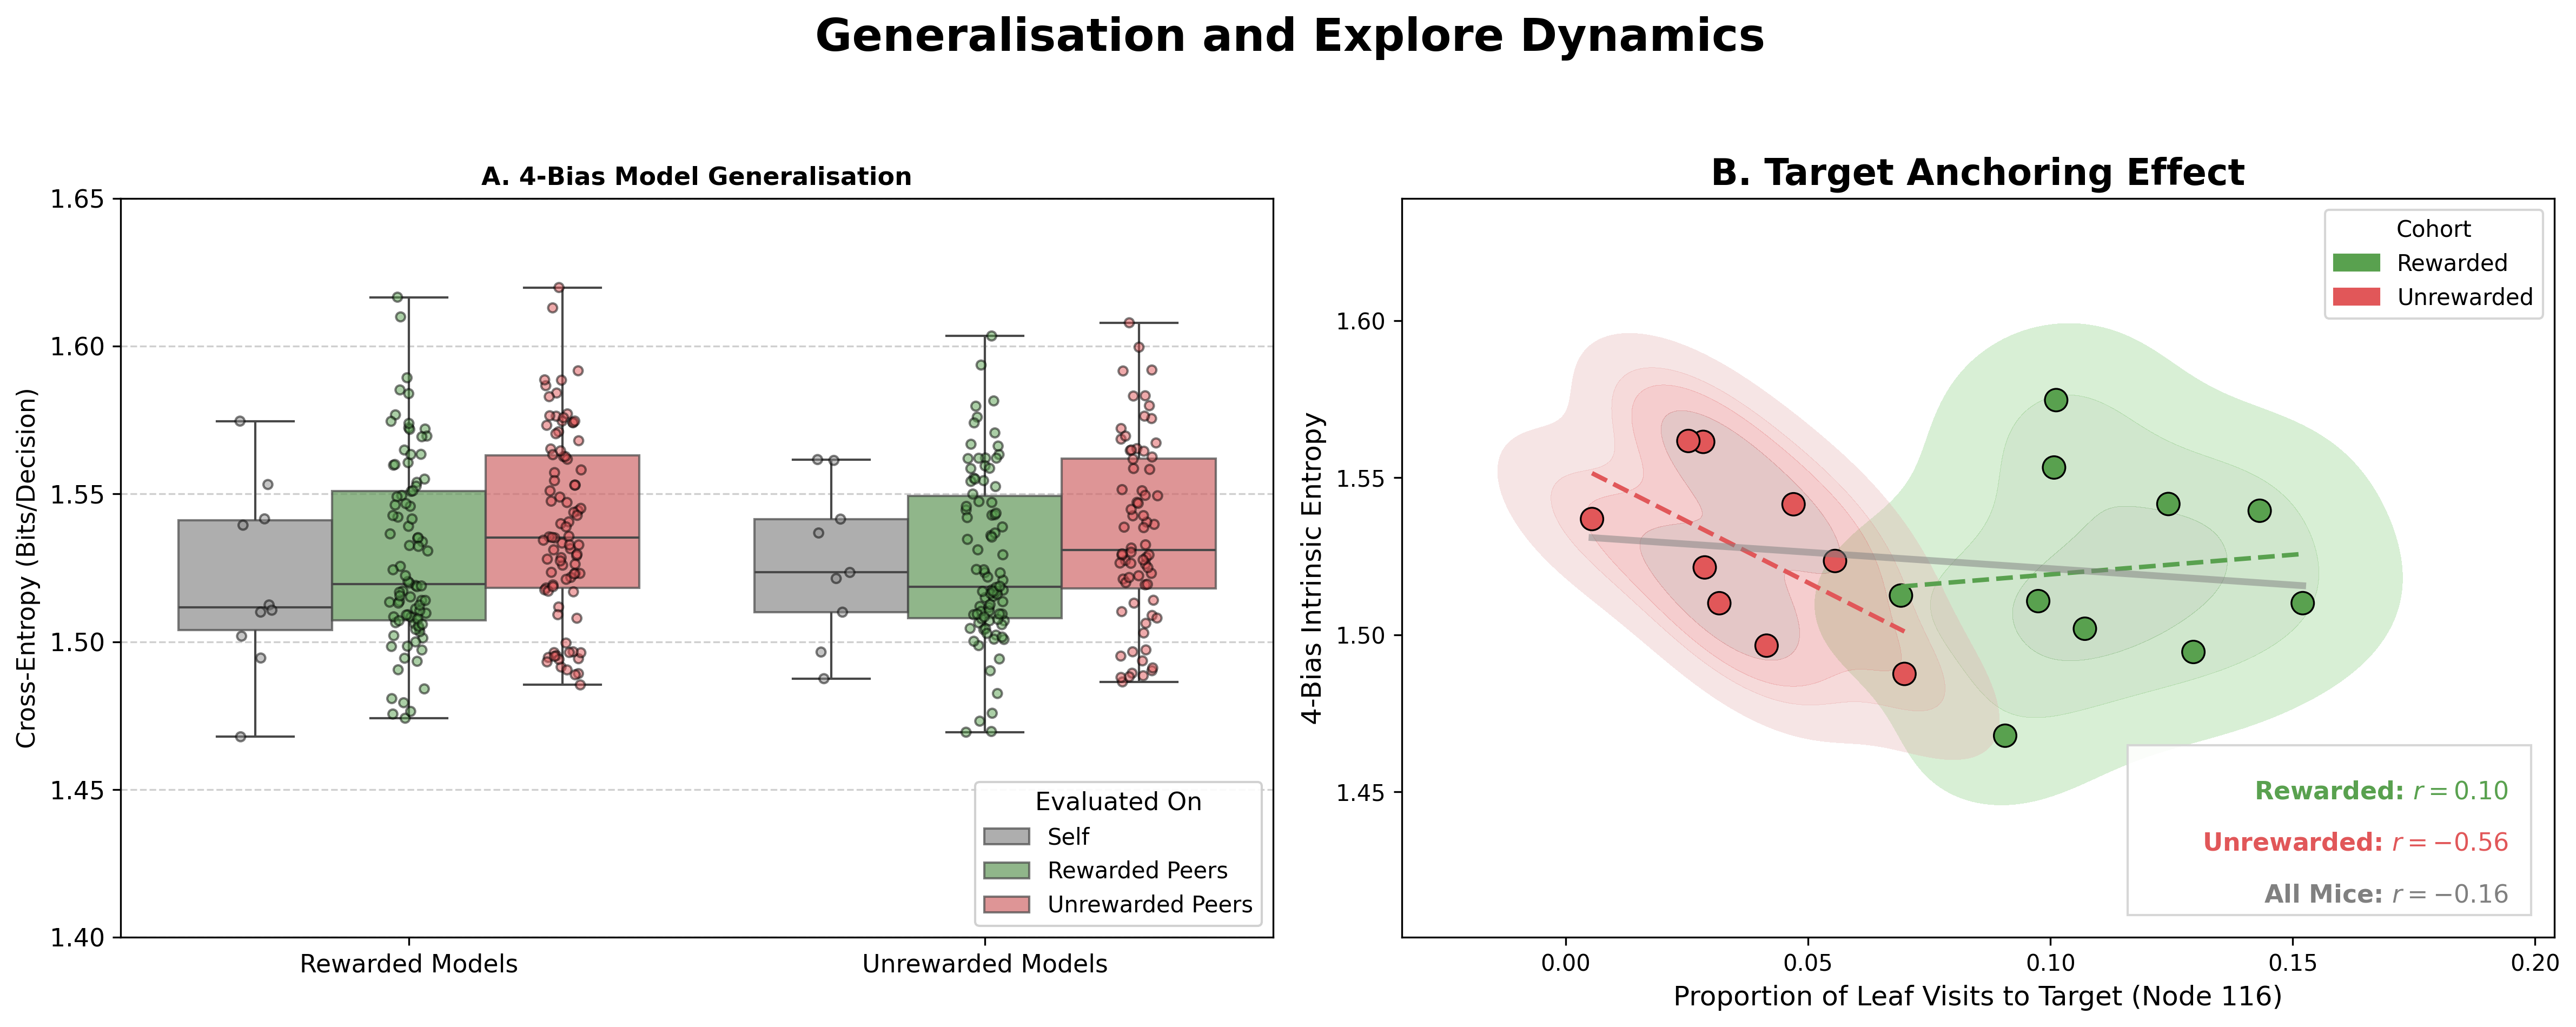
\includegraphics[width=\singlefigure]{figures/generalisation_and_anchoring_box.png}
\end{figure}

\subsection{Does the Water Port Still Matter?}

\begin{itemize}
    \item We revisit the question of whether the water port influences exploration.
    \item We plot the intrinsic entropy of mice (modelled and tested on 100\% of their data) against the proportion of leaf node visits made to the water port node (116).
    \item We note that since modelling is run on the explore mode data, the intrinsic exploration for the rewarded group actually excludes paths to the water port.
    \item As such, the bias should have been removed from modelling, and this is corroborated by the spherical distribution and near zero pearson correlation.
    \item However, visits to the water port have not been removed from the unrewarded mice since they are never in drink mode.
    \item We observe a correlation of -0.56 between the intrinsic exploration and the proportion of water port visits for the unrewarded mice.
    \item The more visits to the water port, the more structured their exploration.
    \item This may be indicative that the short paths, including paths to water port, discussed in <previous section>, and the tendency for mice to investigate node 116, may result in more structured exploration bouts.
    \item In future work, it may be useful to interrogate these more directed explorations, and possibly to classify an aditional behavioural mode which separates this behaviour.
\end{itemize}

\section{Navigation Strategies}

Organisms navigating complex environments face a fundamental trade-off between exploration (gathering information about the environment) and exploitation (using existing knowledge to achieve goals efficiently). This dilemma is particularly seen in spatial navigation, where the value of exploration must be weighed against the time and energy costs of acquiring spatial knowledge that may or may not be useful (Hills et al., 2015; Mehlhorn et al., 2015).

The study of spatial navigation has focused on two strategies:

\begin{itemize}
\item \textbf{Local heuristics:} simple, egocentric rules that guide movement based on immediate sensory input without requiring a global spatial representation (O'Keefe \& Nadel, 1978; Redish, 1999). Examples include wall-following, alternation biases (tendency to alternate left-right turns), and beacon-following. These strategies require minimal memory and can be deployed immediately but may produce suboptimal results in complex environments.

\item \textbf{Cognitive maps:} mental representations of the environment that encode spatial relationships between locations, enabling flexible path planning and shortcuts (Tolman, 1948; O'Keefe \& Nadel, 1978; Moser et al., 2008). Cognitive maps are thought to be implemented in the hippocampal formation through place cells, grid cells, and associated circuits. While enabling efficient navigation, map construction requires extensive exploration and substantial neural investment.
\end{itemize}

The study conducted by Rosenberg et al.\ (2021) provides insight into this exploration behaviour in mice. Water-deprived mice learned to navigate to the hidden water port after only $\approx 10$ reward experiences --- approximately $1000$-fold faster than conventional two-alternative forced choice (2AFC) tasks where thousands of trials are required (Burgess et al., 2017). Despite achieving reliable navigation to the water port, mice spent approximately $84\%$ of their time in the maze exploring rather than executing direct paths to the goal. This proportion was remarkably consistent across animals and persisted even in unrewarded control mice (who spent $95\%$ of time exploring), indicating strong intrinsic motivation for environmental exploration.

The authors stated that the mice often followed local navigation heuristics – alternation bias, branch bias, and forward motion bias – during their exploration. Mice demonstrated accurate homing behavior from their very first deep excursion into the maze, returning directly to the entrance from endpoints without retracing their entry path. The authors suggest this could reflect immediate acquisition of some form of cognitive spatial representation. However, the binary tree structure of the maze used in this study is such that navigating from any node to the entrance did not require memorizing the route. The branch bias – the statistical preference for turning at junctions over continuing straight – is sufficient to guide the animal back to the entrance from any location in the maze. Thus, it remains possible that the mice did not learn a specific path home, but instead relied on this local turning heuristic, which reliably produces successful homing in this particular maze structure.

\subsection{Time Allocation in Navigation}
This extension focuses on identifying the trade-off between maintaining a cognitive map and relying on navigation heuristics. It uses a time-based navigation strategy comparison to calculate how many exploitation episodes are required for the cognitive map to become advantageous. We model strategy selection as a time allocation problem: animals minimize the total time required to complete a fixed number of foraging trips, subject to the constraint that some strategies require upfront temporal investment before achieving efficiency.\\
For a number of exploitation cycles, \textit{N} (number of complete foraging cycles from entrance to water to exit, referred to as \textit{bouts}), the total time for each strategy is:

\begin{itemize}
\item Heuristic strategy:
\[
T_{\text{total}} = N \times t_{\text{heuristic}}
\]

\item Cognitive map strategy:
\[
T_{\text{total}} = T_{\text{learning}} + N \times t_{\text{map}}
\]
\end{itemize}

In the above equations, $t_{\text{heuristic}}$ and $t_{\text{map}}$ represent the average time per trip for each strategy, and $T_{\text{learning}}$ represents the total time invested in exploration to construct the cognitive map. The critical breakeven point $N^*$ occurs where these total times are equal; where strategies yield equal total time:
\[
N^* = \frac{T_{\text{learning}}}{t_{\text{heuristic}} - t_{\text{map}}}
\]

For $N < N^*$, heuristics minimize total time despite being less efficient per trip, because the learning investment cannot be amortized over a sufficiently long exploitation phase. For $N > N^*$, cognitive maps become favorable. Crucially, all quantities in this framework—training time, average trip duration, and breakeven point—are directly measured from simulation rather than assumed, providing a parameter-free comparison grounded in observable behavior.

\subsection{Computational Model}
We implemented 2 agents operating in a binary tree labyrinth (k=2, depth=6) matching the exact structure used by the authors: 63 T-junctions connected by corridors leading to 64 endpoints, one containing a water port. Additionally, we increased the complexity of the labyrinth by increasing the value of the branching factor, \textit{k} and ranging the depth (number of hierarchical levels), \textit{D}, from 3-6.

\subsubsection{Cognitive Map Agent}
Implemented as tabular Q-learning (Watkins \& Dayan, 1992), this agent stores explicit state-action values representing a computational cognitive map.

\subsubsection{Heuristic Agent}
The heuristic agent was implemented using probabilistic navigation rules extracted from Rosenberg et al.'s analysis. This agent followed a decision hierarchy (an order of priorities):
\begin{itemize}
    \item Home run: If find water, reverse and go home by.
    \item Dead end: If reach a dead end, reverse 
    \item Probabilistic exploration: Sampled from the biased action distribution.
\end{itemize}
We set up biased parameters for the heuristics in the action space:
\begin{itemize}
    \item $w_\textit{forward}$ = 2.0 (Bias toward moving ahead rather than reversing)
    \item $w_\textit{alternating}$ = 1.5 (Bias toward alternating left and right turns)
    \item $w_\textit{}$
\end{itemize}

\section{Reward-Based Latent Hazard Model}

Rosenberg et al. (2021) propose computational methods to explain abrupt shifts in behavior in the maze experiment. One possibility is gradual reinforcement learning, where behavioral biases accumulate slowly through repeated reward feedback \cite{sutton2018}. Another possibility is that animals abruptly change their strategies after accumulating sufficient evidence for the optimal path. To explore these possibilities, they expand upon the original Rosenberg modeling framework by comparing three alternative models of learning dynamics: the gradual learning model, the latent hazard model, and the forced insight model.

The behavioral trajectory of a mouse in the maze is represented using a second-order Markov model defined on the maze graph. At each step, the next state depends on the current node, the previous node and a transition probability matrix. The model uses four behavioral bias parameters:
\begin{equation}
b_i = (B_f, B_a, L_f, L_o)
\end{equation}

Where $B_f$ is the probability of moving forward rather than returning to the parent node, $B_a$ is the probability of alternating direction after forward movement, $L_f$ is the probability of leaving a branch rather than backtracking and $L_o$ is the probability of exiting toward the outer maze. These parameters define the transition tensor:
\begin{equation}
T(s_{t-1}, s_t , s_{t+1})
\end{equation}

\subsection{Gradual Learning Model}
The incremental learning model updates behavioral bias using reward-dependent Bayesian updates. After the reward is received, the pseudo-numbers are updated as follows:
\begin{equation}
a_i = a_i + \eta \cdot N_i^{reward}
\end{equation}

\begin{equation}
 b_i = b_i + \eta 
\cdot N_i^{nonreward}
\end{equation}
where:
\begin{itemize}
    \item $a_i, b_i$ are Beta distribution parameters
    \item $\eta$ is the learning rate
    \item $N_i$ represents transition counts
\end{itemize}
Within the model, the Beta distribution restricts transition probabilities to between 0 and 1, providing a natural conjugate prior distribution for Bernoulli processes \cite{bishop2006}.

\subsection{Latent Hazard Insight} 
The Reward-Based Latent Hazard Model, instead of making incremental parameter updates, assumes that insight occurs when sufficient reward evidence accumulates and switches between two behavioral modes:
\begin{equation}
 b^{explore} = (0.778, 0.728, 0.827, 0.655) 
\end{equation}
The exploration parameters correspond to the baseline behavioural biases reported in Rosenberg et al. (2021).
\begin{equation}
b^{exploit} = (0.928, 0.728, 0.907, 0.655)
\end{equation}
The exploitation parameters increase forward and branch-following biases, reflecting more efficient reward-directed navigation after learning.
The probability of switching between these modes depends on the number of rewards observed:
\begin{equation}
p(\text{switch}) = \sigma \left(k (R - \theta)\right)
\label{eq:switch}
\end{equation}

\begin{figure}[htbp]
    \centering
    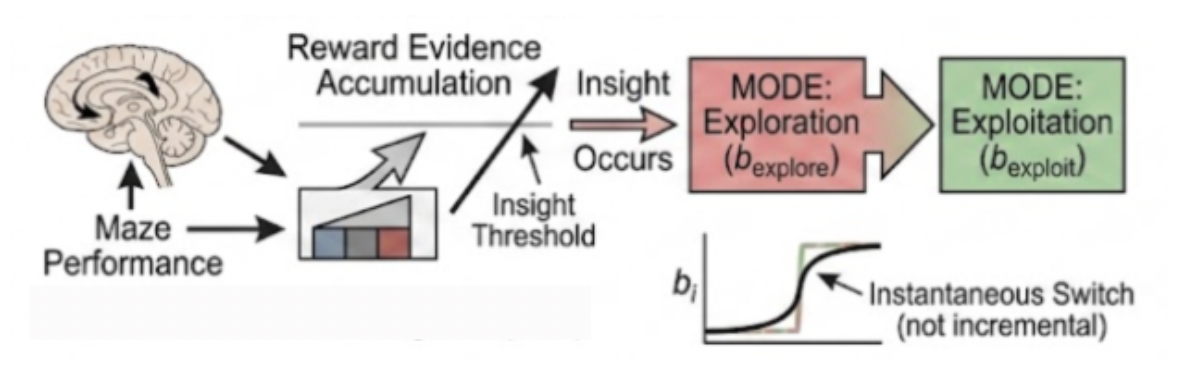
\includegraphics[width=\columnwidth]{figures/pbm_1.png}
    \caption{Schematic of the reward-based latent hazard mechanism: accumulated reward evidence increases the probability of an insight-triggered switch.}
    \label{fig:mechanism}
\end{figure}

To measure model performance, simulated trajectories were compared to the actual mouse trajectory using various goodness-of-fit metrics. 

\begin{figure}[htbp]
    \centering
    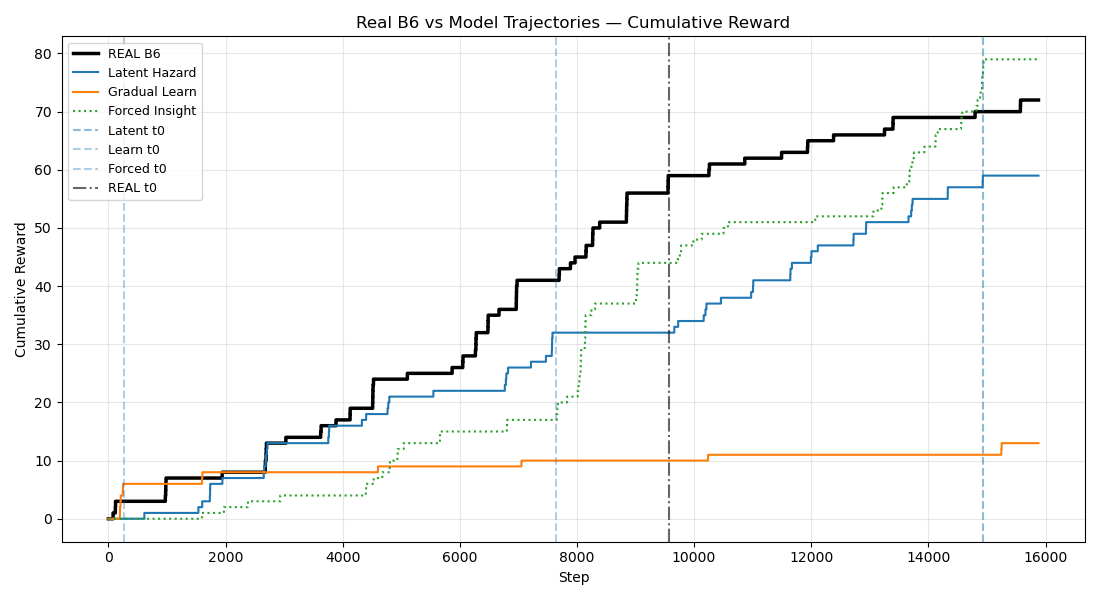
\includegraphics[width=\columnwidth]{figures/pbm_Figure_1.png}
    \caption{Model comparison of cumulative reward trajectories. The graph shows the cumulative reward trajectory of the B6 mouse used in the experiment compared with three simulation models: the Latent Hazard model, the Stepwise Learning model, and the Forced Insight model. The simulations were run with the same trajectory length (15,881 steps) to provide comparable goodness-of-fit assessments. Vertical dashed lines indicate the estimated point of change $(t_0)$ identified using reward rate change point analysis. While the latent hazard model reproduces a reward rate transition similar to the empirical trajectory, the stepwise learning model appears to fail to capture the abrupt behavioral change. The Forced Insight model produces a sharp transition but deviates from the true trajectory in overall reward accumulation.}
    \label{fig:trajectories}
\end{figure}

\begin{table}[htbp]
\centering
\caption{Quantitative Model Fit (Real B6 vs models; $n = 10$ seeds)}
\label{tab:model_fit}
\resizebox{\columnwidth}{!}{%
\begin{tabular}{lcccc}
\hline
Model & $\Delta t_0$ (med [Q1,Q3]) & MSE (mean $\pm$ SD) & $\Delta R_{tot}$ \\
\hline
Latent Hazard & 6134 [4293, 9028] & 130.94 $\pm$ 84.26 & 16.8 $\pm$ 9.4 \\
Gradual Learn & 8704 [8021, 9188] & 1494.56 $\pm$ 162.91 & 58.1 $\pm$ 3.1 \\
Forced Insight & 8247 [4574, 8973] & 71.30 $\pm$ 43.80 & 8.1 $\pm$ 6.9 \\
\hline
\end{tabular}%
}
\end{table}
As shown in Figure 1 and quantified in Table 1, the gradual learning model shows substantially larger trajectory error (MSE), whereas the latent hazard model provides a better overall balance between change-point timing and cumulative trajectory fit.

\subsection{Model Calibration}

To identify biologically plausible parameters for the latent hazard model, 
a grid search was performed over the switching threshold ($\theta$) and 
hazard sharpness parameter ($k$). Candidate parameter values were

\begin{equation}
\theta \in \{6,8,10,12,14\}, \quad
k \in \{0.2,0.4,0.6,0.8\}
\end{equation}

For each parameter pair, simulations were repeated across multiple random 
seeds ($n = 10$). The resulting trajectories were compared with the real 
B6 mouse trajectory using several goodness-of-fit metrics.

To select the best parameter combination, a composite score was constructed 
by normalizing and combining the following metrics:

\begin{itemize}
\item change-point timing error ($\Delta t_0$)
\item reward difference at the transition ($\Delta Reward_{t0}$)
\item cumulative trajectory error (MSE)
\item transition width difference ($\Delta w$)
\item slope ratio difference ($|\Delta \log SR|$)
\end{itemize}

The parameter pair minimizing the composite score was selected as the 
optimal latent hazard configuration.
\subsection{Change-Point Detection}

To estimate the timing of the behavioral transition, we applied a 
change-point detection procedure to the cumulative reward trajectory. 
The reward increment series was smoothed and approximated by a 
two-segment piecewise model representing pre- and post-insight reward rates.

The optimal transition point $t_0$ was defined as the point that minimizes 
the sum of squared errors (SSE) across the two segments:

\begin{equation}
t_0 = \arg\min_{t} (SSE_{pre}(t) + SSE_{post}(t))
\end{equation}

where $SSE_{pre}$ and $SSE_{post}$ represent the squared deviations of the 
reward increments from the estimated reward rate before and after the 
transition point.
\subsection{Transition Width}

To quantify the abruptness of the behavioral transition, we measured the 
transition width ($w$), defined as the interval between the 10\% and 90\% 
increase in the smoothed reward acquisition rate:

\begin{equation}
w = t_{90\%} - t_{10\%}
\end{equation}

Following Rosenberg et al. \cite{rosenberg2021}, transitions with $w < 300$ steps are interpreted as evidence for sudden insight rather than gradual learning.
\subsection{Slope Ratio Metric}

To quantify the increase in reward collection efficiency after insight, 
we computed the slope ratio (SR), defined as the ratio between post-transition 
and pre-transition reward acquisition rates:

\begin{equation}
SR = \frac{r_{post}}{r_{pre}}
\end{equation}

where $r_{pre}$ and $r_{post}$ represent the average reward rates before 
and after the estimated change-point.

For model comparison we evaluated the absolute difference between the 
logarithmic slope ratios of simulated and real trajectories:

\begin{equation}
|\Delta \log SR|
\end{equation}

which captures discrepancies in the magnitude of reward-rate acceleration.
\section{Dopamine Dependent Insight Threshold}
To provide a biological basis for the developed Latent Hazard Model, we integrated the COMT Val158Met polymorphism into the model. The COMT enzyme is responsible for dopamine degradation in the prefrontal cortex (PFC). Neurobiologically, dopamine is known to regulate synaptic plasticity 
through modulation of long-term potentiation (LTP) thresholds in 
prefrontal and hippocampal circuits. Higher tonic dopamine levels 
facilitate synaptic potentiation and reduce the evidence required to 
stabilize a new behavioral strategy.

Within the latent hazard framework, this mechanism can be interpreted 
as a shift in the internal evidence threshold required to trigger the 
exploration–exploitation transition. Consequently, genotypes associated 
with higher dopamine levels should reach the insight transition earlier, 
while genotypes with lower dopamine tone require more accumulated 
reward evidence before switching strategies.The literature shows that the Met allele leads to lower enzyme activity and consequently higher tonic dopamine levels \cite{bilder2004}. 
Neurobiologically, high dopamine levels lower the synaptic potentiation (LTP) threshold, thus increasing learning flexibility. This is expressed in the model by a genotype-dependent scaling factor ($f$):
\begin{equation}
\theta_{bio} = \theta \times f
\end{equation}

\begin{figure*}[t]
    \centering

\includegraphics[width=\textwidth]{A.png}
    \caption{Genotype-dependent differences in insight timing predicted by the latent hazard model. (A) Distribution of simulated insight steps across COMT Val158Met genotypes. Points represent the median insight time across multiple simulation seeds, and error bars indicate the interquartile range (IQR). Higher dopamine levels (Met/Met) correspond to a lower effective switching threshold $\theta$, leading to earlier insight transitions. Conversely, lower dopamine levels (Val/Val) delay the onset of insight. (B) Median cumulative reward trajectories for each genotype. Curves represent the median trajectory across seeds for the latent hazard model. Vertical dashed lines indicate the estimated insight transition point for each genotype. Increasing the biological threshold $\theta_{bio} = \theta \times f$ shifts the exploration–exploitation transition to later steps, producing systematically delayed learning in the low-dopamine condition.}
    \label{fig:genotype_results}
\end{figure*}

In the simulations, genotype effects were implemented by scaling the 
switching threshold parameter $\theta$ using the genotype-dependent 
factor $f$. This modification changes the amount of accumulated reward 
evidence required before the exploration–exploitation transition occurs, 
thereby shifting the timing of the insight event.
This formulation allows dopamine-dependent genetic variation to directly 
modulate the evidence threshold for insight. In this framework, lower 
values of $\theta_{bio}$ increase the probability of earlier switching 
according to the switching rule defined in
according to the switching rule defined in Equation~\ref{eq:switch}. 

Substituting the biological threshold $\theta_{bio}$ shifts the sigmoid 
switching function toward lower reward counts, effectively predicting 
earlier exploration–exploitation transitions for high-dopamine genotypes.

Thus, higher dopamine levels effectively shift the sigmoid switching 
curve toward earlier reward counts.



\begin{table}[htbp]
\centering
\caption{Genotype-dependent Scaling Factors}
\label{tab:genotypes}
\begin{tabular}{lcc}
\toprule
\textbf{Genotype} & \textbf{Dopamine Level} & \textbf{Scaling Factor (f)} \\
\midrule
Met/Met & High    & 0.6 \\
Val/Met & Normal  & 1.0 \\
Val/Val & Low     & 1.4 \\
\bottomrule
\end{tabular}
\end{table}


Simulation results (n = 10 seeds; median [Q1, Q3]) show that dopamine-dependent shifts in the switching threshold strongly influence insight timing. The high-dopamine genotype (Met/Met) reaches insight at approximately step 1972 with the lowest effective threshold $(\theta_{bio}=8.4)$, producing the earliest transition to exploitation. In contrast, the low-dopamine genotype (Val/Val), associated with higher COMT activity and reduced dopaminergic tone, reaches insight much later at approximately step 3904 $(\theta_{bio}=19.6)$. This genotype-dependent separation is clearly visible in Figure 3 as a systematic shift of the exploration–exploitation transition toward later steps.
The logarithmic slope ratio $(log_SR)$ analysis shows that all three genotypes increase the reward collection rate after insight. The fact that the $Low_DA$ group had the highest $log_SR$ value (0.960) may indicate that the behavioral effect of the insight, even if delayed, is quite strong.
% \input{sections/results}
% \input{sections/conclusions}

% BIBLIOGRAPHY
\appendix
\bibliography{references}

\end{document}